% ============================================================
%  LAPORAN RANCANG BANGUN SISTEM ANDROMEDA
%  ANDROMEDA - Android Routine Monitoring Electronic Drip Automation
%  Sistem Irigasi Tetes Otomatis Berbasis IoT
%  dengan Monitoring dan Kontrol Flutter
% ============================================================
\documentclass[12pt,a4paper,oneside]{report}

% --- Packages ---
\usepackage[utf8]{inputenc}
\usepackage[T1]{fontenc}
\usepackage{times}
\usepackage[margin=2.5cm,top=3cm,bottom=3cm]{geometry}
\usepackage{graphicx}
\usepackage{float}
\usepackage{tikz}
\usetikzlibrary{shapes,arrows,positioning,decorations.pathreplacing,calc,fit}
\usepackage{booktabs}
\usepackage{longtable}
\usepackage{array}
\usepackage{multirow}
\usepackage{caption}
\usepackage{xcolor}
\usepackage{hyperref}
\usepackage{setspace}
\usepackage{enumitem}
\usepackage{titlesec}
\usepackage{chngcntr}
\usepackage{lipsum}
\usepackage{fancyhdr}
\usepackage{indentfirst}
\usepackage{pifont}
\usepackage{listings}
\usepackage{tabularx}

% --- Color definitions ---
\definecolor{primaryblue}{RGB}{0,102,204}
\definecolor{accentgreen}{RGB}{0,153,76}
\definecolor{lightgray}{RGB}{245,245,245}
\definecolor{darkgray}{RGB}{50,50,50}

% --- Hyperlink setup ---
\hypersetup{
    colorlinks=true,
    linkcolor=primaryblue,
    urlcolor=primaryblue,
    citecolor=primaryblue
}

% --- Page style ---
\pagestyle{fancy}
\fancyhf{}
\fancyhead[L]{\small \textit{Sistem Irigasi Tetes Otomatis Berbasis IoT}}
\fancyhead[R]{\small \thepage}
\renewcommand{\headrulewidth}{0.4pt}

% --- Section formatting ---
\titleformat{\chapter}{\Large\bfseries\color{primaryblue}}{BAB \thechapter}{0.5em}{\large\bfseries}
\titlespacing*{\chapter}{0pt}{-20pt}{20pt}

\titleformat{\section}{\large\bfseries}{\thesection}{0.5em}{}
\titleformat{\subsection}{\bfseries}{\thesubsection}{0.5em}{}

% --- Spacing ---
\onehalfspacing

% --- Listings style ---
\lstdefinestyle{custom}{
    backgroundcolor=\color{lightgray},
    basicstyle=\footnotesize\ttfamily,
    breaklines=true,
    frame=single,
    numbers=left,
    numberstyle=\tiny,
    xleftmargin=2em
}

% ============================================================
%  DOCUMENT START
% ============================================================
\begin{document}

% --- Cover ---
\begin{titlepage}
\begin{center}

\vspace*{1cm}


\begin{tikzpicture}
\shadedraw[top color=primaryblue!20,bottom color=primaryblue!80,draw=primaryblue,rounded corners=8pt]
(0,0) rectangle (14,2.5);
\node[text=white,font=\bfseries\Huge] at (7,1.25) {LAPORAN RANCANG BANGUN};
\end{tikzpicture}

\vspace{0.3cm}


\begin{tikzpicture}
\shadedraw[top color=accentgreen!20,bottom color=accentgreen!80,draw=accentgreen,rounded corners=8pt]
(0,0) rectangle (14,2.5);
\node[text=white,font=\bfseries\Huge] at (7,1.25) {SISTEM IRIGASI TETES OTOMATIS};
\end{tikzpicture}

\vspace{0.3cm}

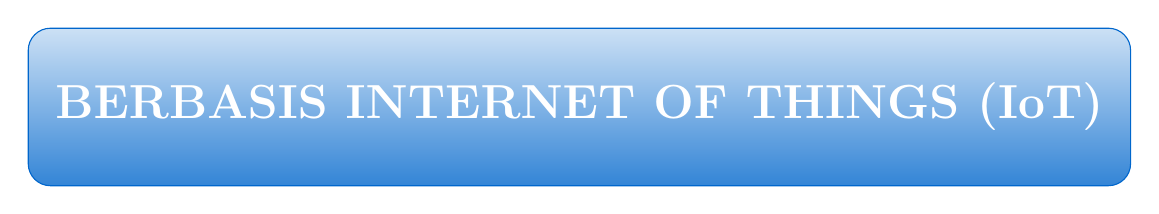
\begin{tikzpicture}
\shadedraw[top color=primaryblue!20,bottom color=primaryblue!80,draw=primaryblue,rounded corners=8pt]
(0,0) rectangle (14,2.0);
\node[text=white,font=\bfseries\LARGE] at (7,1.0) {BERBASIS INTERNET OF THINGS (IoT)};
\end{tikzpicture}

\vspace{0.3cm}


\begin{tikzpicture}
\shadedraw[top color=accentgreen!20,bottom color=accentgreen!80,draw=accentgreen,rounded corners=8pt]
(0,0) rectangle (14,1.5);
\node[text=white,font=\bfseries\large] at (7,0.75) {DENGAN MONITORING DAN KONTROL BERBASIS FLUTTER};
\end{tikzpicture}

\vspace{1.5cm}

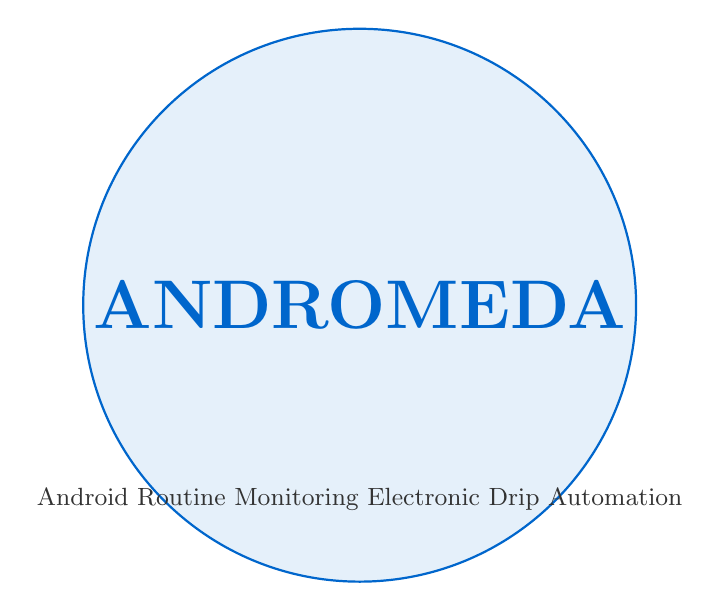
\begin{tikzpicture}
\node[circle,draw=primaryblue,thick,fill=primaryblue!10,minimum size=3.5cm,font=\bfseries\Huge\color{primaryblue}] {ANDROMEDA};
\node[below,font=\small\color{darkgray}] at (0,-2.2) {Android Routine Monitoring Electronic Drip Automation};
\end{tikzpicture}

\vspace{2cm}

{\large
\textbf{Disusun Oleh:}\\[0.3cm]
\textbf{Farrel Ghozy Afifudin}\\[0.1cm]
NIM: 452024611053
}

\vspace{1.5cm}

{\large
\textbf{PROGRAM STUDI TEKNIK INFORMATIKA}\\[0.1cm]
\textbf{UNIVERSITAS DARUSSALAM GONTOR}\\[0.1cm]
\textbf{2025}}
\end{center}
\end{titlepage}

% --- Kata Pengantar ---
\chapter*{KATA PENGANTAR}
\addcontentsline{toc}{chapter}{KATA PENGANTAR}

Puji syukur ke hadirat Allah SWT atas segala rahmat dan hidayah-Nya sehingga laporan rancang bangun \textit{Sistem Irigasi Tetes Otomatis Berbasis Internet of Things (IoT) dengan Monitoring dan Kontrol Berbasis Flutter} ini dapat diselesaikan dengan baik.

Laporan ini disusun sebagai dokumen perencanaan teknis untuk pengembangan sistem irigasi cerdas yang mengintegrasikan sensor kelembaban tanah, mikrokontroler ESP32, aktuator solenoid valve, serta aplikasi Flutter untuk monitoring dan kontrol secara \textit{real-time}. Sistem ini dirancang untuk mengoptimalkan penyiraman tanaman — khususnya benih padi, cabai, dan tanaman hortikultura lainnya — secara otomatis berdasarkan kondisi kelembaban tanah aktual.

Kami menyadari bahwa laporan ini masih jauh dari sempurna. Oleh karena itu, kritik dan saran yang membangun sangat diharapkan untuk pengembangan lebih lanjut. Semoga laporan ini dapat memberikan manfaat dan menjadi referensi yang berguna dalam pengembangan sistem irigasi cerdas di masa mendatang.

\vspace{1cm}
\begin{flushright}
Gontor, 2025

Penulis
\end{flushright}

% --- Daftar Isi ---
\newpage
\tableofcontents
\newpage

\listoffigures
\listoftables

% ============================================================
%  BAB I  -  PENDAHULUAN
% ============================================================
\chapter{PENDAHULUAN}

\section{Latar Belakang}

Pertanian dan perkebangan merupakan sektor vital dalam perekonomian Indonesia. Namun, sebagian besar petani masih menggunakan metode penyiraman konvensional yang kurang efisien — baik dari segi penggunaan air, tenaga kerja, maupun waktu. Penyiraman manual seringkali mengakibatkan pemborosan air karena tidak memperhitungkan kondisi kelembaban tanah yang sebenarnya.

Perkembangan teknologi \textit{Internet of Things} (IoT) membuka peluang baru dalam sektor pertanian presisi (\textit{precision agriculture}). Dengan menghubungkan sensor, aktuator, dan perangkat komputasi ke jaringan internet, maka monitoring dan kontrol lahan pertanian dapat dilakukan secara \textit{real-time} dari jarak jauh melalui perangkat seluler seperti smartphone.

Berdasarkan permasalahan tersebut, proyek \textbf{ANDROMEDA (Android Routine Monitoring Electronic Drip Automation)} dirancang sebagai sistem irigasi tetes otomatis yang mampu:
\begin{enumerate}
    \item Memantau kondisi kelembaban tanah secara \textit{real-time}.
    \item Mengaktifkan penyiraman secara otomatis ketika kelembaban berada di bawah ambang batas.
    \item Memberikan kontrol manual melalui aplikasi Flutter.
    \item Menyediakan data historis untuk analisis pola penyiraman.
\end{enumerate}

Dengan sistem ini, diharapkan penggunaan air menjadi lebih efisien, tanaman tumbuh optimal, dan petani dapat memonitor lahannya kapan saja dan di mana saja.

\section{Rumusan Masalah}

Berdasarkan latar belakang di atas, rumusan masalah dalam proyek ini adalah sebagai berikut:
\begin{enumerate}
    \item Bagaimana merancang sistem irigasi tetes otomatis yang dapat mengukur kelembaban tanah secara \textit{real-time}?
    \item Bagaimana mengintegrasikan sensor kelembaban tanah dengan mikrokontroler ESP32 dan aktuator solenoid valve?
    \item Bagaimana membangun sistem komunikasi data dari perangkat keras ke aplikasi melalui HTTP REST ke Supabase?
    \item Bagaimana merancang aplikasi Flutter untuk monitoring dan kontrol sistem irigasi?
\end{enumerate}

\section{Tujuan}

Tujuan dari proyek ANDROMEDA ini adalah:
\begin{enumerate}
    \item Merancang dan membangun sistem irigasi tetes otomatis berbasis IoT yang terintegrasi dengan sensor kelembaban tanah.
    \item Mengimplementasikan mikrokontroler ESP32 sebagai pengendali utama sistem yang terhubung ke internet melalui WiFi.
    \item Mengembangkan aplikasi Flutter untuk monitoring kondisi tanah dan kontrol penyiraman secara \textit{real-time}.
    \item Menghasilkan dokumentasi teknis yang lengkap sebagai referensi pengembangan lebih lanjut.
\end{enumerate}

\section{Manfaat}

Manfaat yang diharapkan dari proyek ANDROMEDA:
\begin{enumerate}
    \item \textbf{Efisiensi Air} — Penyiraman dilakukan hanya saat dibutuhkan berdasarkan data kelembaban aktual, mengurangi pemborosan air hingga 30-50\%.
    \item \textbf{Optimasi Pertumbuhan Tanaman} — Tanaman mendapat suplai air yang konsisten dan sesuai kebutuhan.
    \item \textbf{Penghematan Tenaga Kerja} — Sistem bekerja otomatis tanpa perlu pengawasan manual terus-menerus.
    \item \textbf{Monitoring Jarak Jauh} — Petani dapat memantuk kondisi lahan dari mana saja melalui smartphone.
    \item \textbf{Data Historis} — Data kelembaban tersimpan untuk analisis pola dan evaluasi.
\end{enumerate}

\section{Batasan Masalah}

Batasan masalah dalam proyek ini meliputi:
\begin{enumerate}
    \item Sistem dirancang untuk 1 titik tanam (1m × 7m) dengan 1 sensor dan 1 solenoid valve.
    \item Konektivitas menggunakan WiFi — sistem hanya berfungsi di area dengan akses internet.
    \item Sumber daya listrik menggunakan aki 100Ah + solar panel 300Wp (off-grid, mandiri energi).
    \item Sensor yang digunakan adalah sensor kelembaban tanah kapasitif (\textit{capacitive soil sensor}).
    \item Aktuator yang digunakan adalah solenoid valve 12V NC dengan selang drip \textit{irrigation}.
    \item Aplikasi dikembangkan menggunakan Flutter (Dart) dengan Supabase SDK dan REST API.
    \item Sistem belum mencakup pengaturan pH tanah atau nutrisi tanaman.
\end{enumerate}


% ============================================================
%  BAB II - TINJAUAN PUSTAKA
% ============================================================
\chapter{TINJAUAN PUSTAKA}

\section{Internet of Things (IoT)}

\textit{Internet of Things} (IoT) merupakan konsep di mana objek fisik (\textit{things}) dilengkapi dengan sensor, aktuator, dan konektivitas jaringan sehingga dapat saling bertukar data melalui internet. Dalam konteks pertanian, IoT memungkinkan otomatisasi irigasi berdasarkan data sensor \textit{real-time}, bukan berdasarkan jadwal tetap atau perkiraan.

Arsitektur IoT umumnya terdiri dari tiga lapisan:
\begin{enumerate}
    \item \textbf{Perception Layer} — Sensor dan aktuator yang berinteraksi langsung dengan lingkungan fisik.
    \item \textbf{Network Layer} — Infrastruktur komunikasi (WiFi, MQTT, HTTP) yang menghubungkan perangkat ke server.
    \item \textbf{Application Layer} — Aplikasi pengguna (Flutter app, dashboard web) untuk visualisasi dan kontrol.
\end{enumerate}

\begin{figure}[H]
\centering
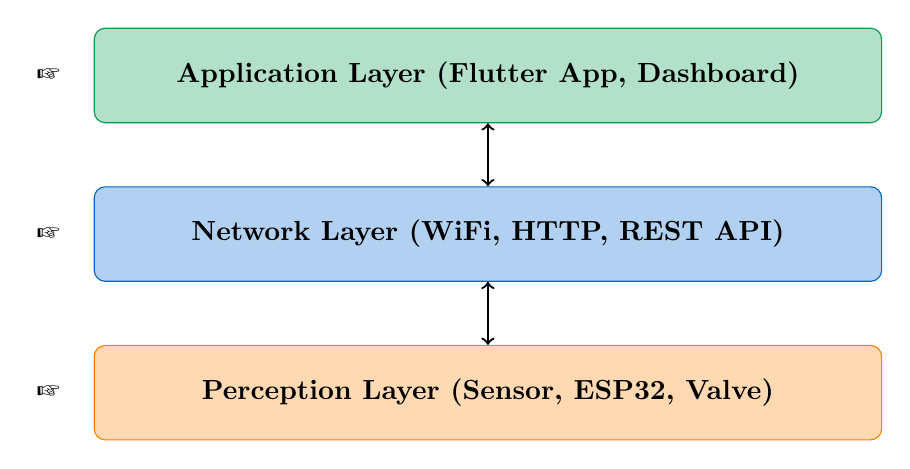
\begin{tikzpicture}[node distance=0.8cm, auto]
    \tikzstyle{layer} = [rectangle, rounded corners, minimum width=10cm, minimum height=1.2cm, text centered, font=\bfseries];

    \node (app) [layer, fill=accentgreen!30, draw=accentgreen] {Application Layer (Flutter App, Dashboard)};
    \node (net) [layer, fill=primaryblue!30, draw=primaryblue, below=of app] {Network Layer (WiFi, HTTP, REST API)};
    \node (per) [layer, fill=orange!30, draw=orange, below=of net] {Perception Layer (Sensor, ESP32, Valve)};

    \draw[<->, thick] (app) -- (net);
    \draw[<->, thick] (net) -- (per);

    \node[left=0.3cm of app, font=\small] {\ding{43}};
    \node[left=0.3cm of net, font=\small] {\ding{43}};
    \node[left=0.3cm of per, font=\small] {\ding{43}};
\end{tikzpicture}
\caption{Arsitektur tiga lapis IoT}
\label{fig:iot-arch}
\end{figure}

\section{Sensor Kelembaban Tanah}

Sensor kelembaban tanah adalah perangkat yang mengukur kadar air dalam tanah. Terdapat dua jenis utama yang umum digunakan dalam proyek IoT:

\subsection{YL-69 (Resistive Soil Sensor)}

Sensor resistif mengukur kelembaban berdasarkan perubahan resistansi listrik antara dua elektroda yang ditancapkan ke tanah. Ketika tanah basah, resistansi menurun (konduktivitas meningkat).

\textbf{Spesifikasi:}
\begin{itemize}
    \item Tegangan operasi: 3.3V -- 5V DC
    \item Output: Analog (0 -- 3.3V) dan Digital (komparator LM393)
    \item Prinsip kerja: Resistif (konduktivitas listrik)
    \item Dimensi: 6.3cm × 2.0cm
    \item Harga: Rp 5.000 -- Rp 15.000
\end{itemize}

\textbf{Kelebihan:}
\begin{itemize}
    \item Harga sangat murah
    \item Mudah ditemukan di pasaran
    \item Respons cepat terhadap perubahan kelembaban
\end{itemize}

\textbf{Kekurangan:}
\begin{itemize}
    \item Elektroda mudah terkorosi karena arus listrik langsung dan reaksi elektrokimia dengan tanah dan air
    \item Akurasi menurun seiring waktu akibat korosi
    \item Masa pakai relatif pendek (3--6 bulan dalam penggunaan terus-menerus)
    \item Tidak cocok untuk penggunaan jangka panjang
\end{itemize}

\subsection{Capacitive Soil Sensor v1.2}

Sensor kapasitif mengukur kelembaban berdasarkan perubahan konstanta dielektrik tanah yang memengaruhi kapasitansi antara dua pelat sensor. Tidak ada kontak listrik langsung dengan tanah, sehingga lebih tahan korosi.

\textbf{Spesifikasi:}
\begin{itemize}
    \item Tegangan operasi: 3.3V -- 5V DC
    \item Output: Analog (0 -- 3.3V)
    \item Prinsip kerja: Kapasitif (perubahan dielektrik)
    \item Dimensi: 9.8cm × 2.3cm
    \item Harga: Rp 25.000 -- Rp 40.000
\end{itemize}

\textbf{Kelebihan:}
\begin{itemize}
    \item Tidak ada kontak listrik langsung dengan tanah $\rightarrow$ anti korosi
    \item Masa pakai jauh lebih panjang (tahun)
    \item Akurasi stabil dalam jangka panjang
    \item Konsumsi daya rendah
    \item Tidak memerlukan kalibrasi ulang berkala
\end{itemize}

\textbf{Kekurangan:}
\begin{itemize}
    \item Harga lebih mahal dibanding YL-69
    \item Respons sedikit lebih lambat (perubahan kapasitansi vs resistansi)
    \item Ukuran fisik sedikit lebih besar
\end{itemize}

\subsection{Perbandingan Sensor Kelembaban Tanah}

\begin{table}[H]
\centering
\caption{Perbandingan Sensor Kelembaban Tanah}
\label{tab:sensor-compare}
\begin{tabular}{p{3.5cm} p{5cm} p{5cm}}
\toprule
\textbf{Parameter} & \textbf{YL-69 (Resistif)} & \textbf{Capacitive Sensor} \\
\midrule
Prinsip Kerja & Resistansi listrik & Kapasitansi dielektrik \\
Ketahanan Korosi & Rendah (korosi cepat) & Tinggi (tanpa kontak langsung) \\
Masa Pakai & 3--6 bulan & $>$ 2 tahun \\
Akurasi Jangka Panjang & Menurun & Stabil \\
Harga & Rp 5.000 -- 15.000 & Rp 25.000 -- 40.000 \\
Respons & Cepat (ms) & Sedang (ms -- detik) \\
Konsumsi Daya & ∼10 mA & ∼5 mA \\
Perawatan & Kalibrasi berkala & Minimal \\
Ketersediaan & Sangat mudah & Mudah \\
Kesesuaian Jangka Panjang & Tidak cocok & Sangat cocok \\
\bottomrule
\end{tabular}
\end{table}

\textbf{Keputusan:} Proyek ANDROMEDA menggunakan \textbf{Capacitive Soil Sensor v1.2} karena:
\begin{enumerate}
    \item Ketahanan jangka panjang — sistem dirancang untuk beroperasi terus-menerus.
    \item Tidak perlu kalibrasi ulang — mengurangi perawatan.
    \item Akurasi stabil — data yang konsisten untuk logika kontrol otomatis.
    \item Investasi jangka panjang lebih murah dibanding mengganti YL-69 setiap 3-6 bulan.
\end{enumerate}

\section{Mikrokontroler}

Mikrokontroler adalah otak dari sistem IoT yang bertugas membaca sensor, memproses data, dan mengendalikan aktuator. Tiga pilihan utama yang umum digunakan:

\subsection{ESP32}

ESP32 adalah mikrokontroler buatan Espressif Systems yang dilengkapi dengan WiFi dan Bluetooth terintegrasi. Ini adalah penerus dari ESP8266 dengan performa yang jauh lebih baik.

\textbf{Spesifikasi:}
\begin{itemize}
    \item CPU: Xtensa dual-core 32-bit LX6 @ 160--240 MHz
    \item SRAM: 520 KB
    \item Flash: 4 MB -- 16 MB
    \item WiFi: 802.11 b/g/n (2.4 GHz)
    \item Bluetooth: v4.2 BR/EDR + BLE
    \item GPIO: 34 pin (dengan ADC, DAC, touch, PWM, I2C, SPI, UART)
    \item ADC: 2x 12-bit (18 channel)
    \item Harga: Rp 50.000 -- Rp 80.000
\end{itemize}

\textbf{Kelebihan:}
\begin{itemize}
    \item Dual-core, performa tinggi untuk multi-tasking
    \item WiFi + Bluetooth dalam satu chip
    \item ADC 12-bit (resolusi lebih tinggi dari ESP8266)
    \item Banyak GPIO untuk ekspansi sensor/aktuator
    \item Mendukung OTA (\textit{Over-the-Air}) update
    \item Komunitas besar dan dokumentasi lengkap
\end{itemize}

\subsection{ESP8266}

ESP8266 adalah pendahulu ESP32 yang juga populer di kalangan penggemar IoT.

\textbf{Spesifikasi:}
\begin{itemize}
    \item CPU: Xtensa single-core 32-bit L106 @ 80 MHz
    \item SRAM: 160 KB (80 KB usable)
    \item Flash: 1 MB -- 4 MB
    \item WiFi: 802.11 b/g/n
    \item GPIO: 17 pin (dengan ADC, PWM, I2C, SPI, UART)
    \item ADC: 1x 10-bit
    \item Harga: Rp 25.000 -- Rp 50.000
\end{itemize}

\textbf{Kekurangan:}
\begin{itemize}
    \item Single-core, kemampuan multitasking terbatas
    \item ADC 10-bit (resolusi lebih rendah)
    \item Hanya 1 channel ADC (tidak bisa multiple sensor analog)
    \item Tidak ada Bluetooth
    \item Tidak mendukung OTA dengan mudah
\end{itemize}

\subsection{Arduino Uno}

Arduino Uno adalah board mikrokontroler klasik berbasis ATmega328P yang sangat populer untuk pembelajaran.

\textbf{Spesifikasi:}
\begin{itemize}
    \item CPU: ATmega328P 8-bit @ 16 MHz
    \item SRAM: 2 KB
    \item Flash: 32 KB
    \item GPIO: 14 pin (6x PWM, 6x ADC 10-bit)
    \item Tidak ada WiFi/Bluetooth bawaan (perlu shield tambahan)
    \item Harga: Rp 60.000 -- Rp 120.000 (asli) / Rp 25.000 -- Rp 40.000 (clone)
\end{itemize}

\textbf{Kekurangan:}
\begin{itemize}
    \item Tidak ada konektivitas nirkabel bawaan (perlu shield tambahan)
    \item Memory sangat terbatas (2 KB SRAM)
    \item Clock speed rendah (16 MHz)
    \item Tidak cocok untuk aplikasi IoT yang terhubung internet
\end{itemize}

\subsection{Perbandingan Mikrokontroler}

\begin{table}[H]
\centering
\caption{Perbandingan Mikrokontroler untuk IoT}
\label{tab:mcu-compare}
\begin{tabular}{p{2.5cm} p{3.5cm} p{3.5cm} p{3.5cm}}
\toprule
\textbf{Parameter} & \textbf{ESP32} & \textbf{ESP8266} & \textbf{Arduino Uno} \\
\midrule
CPU & Dual-core 240 MHz & Single-core 80 MHz & 8-bit 16 MHz \\
SRAM & 520 KB & 160 KB & 2 KB \\
WiFi & Bawaan & Bawaan & Tidak ada \\
Bluetooth & Ada & Tidak ada & Tidak ada \\
ADC & 12-bit (18 ch) & 10-bit (1 ch) & 10-bit (6 ch) \\
GPIO & 34 pin & 17 pin & 14 pin \\
Harga & Rp 50-80rb & Rp 25-45rb & Rp 25-120rb \\
IoT Ready & Sangat cocok & Cukup & Tidak langsung \\
\bottomrule
\end{tabular}
\end{table}

\textbf{Keputusan:} Proyek ANDROMEDA menggunakan \textbf{ESP32} karena:
\begin{enumerate}
    \item WiFi + Bluetooth terintegrasi — tidak perlu modul tambahan.
    \item Dual-core — mampu menjalankan multiple task (baca sensor, kirim data, kontrol valve) secara simultan.
    \item ADC 12-bit resolusi tinggi — menghasilkan data kelembaban yang lebih presisi.
    \item Banyak GPIO — memungkinkan penambahan sensor/aktuator di masa depan.
    \item OTA update — firmware dapat diperbarui dari jarak jauh tanpa harus melepas perangkat.
\end{enumerate}

\section{Aktuator: Solenoid Valve (Rekomendasi)}

Pemilihan aktuator untuk sistem irigasi tetes sangat memengaruhi kinerja dan keandalan sistem. Karena di lokasi tanam Desa Merayan sudah tersedia \textbf{tandon air} beserta \textbf{alat pengisi air otomatis}, pendekatan paling efisien adalah memanfaatkan tekanan gravitasi dari tandon, bukan menggunakan pompa tambahan.

\subsection{Solenoid Valve 12V NC (\textit{Normally Closed})}

Solenoid valve adalah katup listrik yang membuka atau menutup aliran air berdasarkan sinyal listrik. Tipe NC (\textit{Normally Closed}) berarti katup dalam keadaan tertutup saat tidak diberi tegangan, dan terbuka hanya saat relay ESP32 mengaktifkannya. Ini penting untuk \textbf{pengamanan}: jika ESP32 mati atau kehilangan daya, valve otomatis tertutup (fail-safe).

\textbf{Spesifikasi:}
\begin{itemize}
    \item Tegangan: 12V DC
    \item Tipe: Normally Closed (NC)
    \item Tekanan kerja: 0.02 -- 0.8 MPa (cocok untuk gravitasi tandon)
    \item Diameter: 1/2 inch (kran air standar)
    \item Konsumsi daya: ≈500 mA (hanya saat aktif)
    \item Harga: Rp 40.000 -- Rp 60.000
\end{itemize}

\textbf{Kelebihan:}
\begin{itemize}
    \item \textbf{Tidak perlu pompa} — memanfaatkan gravitasi dari tandon yang sudah ada
    \item \textbf{Hemat daya} — konsumsi 0 mA saat valve tertutup, hanya ∼500 mA saat aktif (siram 30 detik = 0.004 Ah\footnote{Perhitungan: 500 mA × 30 detik / 3600 = 0,004 Ah per siklus siram. Dengan 12 siklus/hari = 0,05 Ah/hari. Aki 100Ah bisa bertahan 2.000 hari \textbf{hanya untuk valve}.})
    \item \textbf{Fail-safe} — NC valve otomatis tertutup saat mati listrik, tidak ada banjir
    \item \textbf{Sirkuit sederhana} — cukup relay 1 channel, tidak perlu driver motor
    \item \textbf{Perawatan minimal} — tanpa motor, tanpa sikat karbon, tanpa keausan mekanik
    \item \textbf{Pemasangan mudah} — bisa langsung disambung ke pipa/selang tandon yang sudah ada
\end{itemize}

\subsection{Perbandingan: Solenoid Valve vs Pompa DC}

\begin{table}[H]
\centering
\caption{Perbandingan Solenoid Valve dan Pompa DC untuk sistem irigasi tetes}
\label{tab:actuator-compare}
\begin{tabularx}{\textwidth}{l X X}
\toprule
\textbf{Parameter} & \textbf{Solenoid Valve 12V NC 🔥} & \textbf{Pompa Air DC Mini} \\
\midrule
Biaya & Rp 40.000 -- 60.000 & Rp 25.000 -- 60.000 \\
Prinsip kerja & Membuka/menutup aliran (gravitasi) & Memompa air (tekanan aktif) \\
Daya aktif & \textbf{500 mA} (saat siram saja) & \textbf{200-1000 mA} (selama siram) \\
Daya idle & \textbf{0 mA} ✅ & 0 mA \\
Fail-safe & ✅ Otomatis tertutup saat mati listrik & × Air tetap mengalir jika pompa di ON \\
Kompleksitas & Sederhana (relay) & Sederhana (relay) \\
Cocok tandon? & \textbf{✅ Sangat cocok} & ⚠️ Boros daya \\
Perawatan & Minimal (tidak ada bagian bergerak) & Sikat karbon aus, seal bocor \\
\bottomrule
\end{tabularx}
\end{table}

\textbf{Keputusan:} Proyek ANDROMEDA menggunakan \textbf{Solenoid Valve 12V NC} karena memanfaatkan tandon air yang sudah tersedia, lebih hemat daya (0 mA saat idle, hanya aktif saat menyiram), fail-safe (otomatis tertutup saat mati listrik), dan tidak memerlukan komponen tambahan yang rumit. Dengan sirkuit yang hanya terdiri dari relay ESP32 dan solenoid valve, sistem menjadi lebih sederhana, lebih andal, dan lebih efisien secara energi dibandingkan menggunakan pompa.

\textbf{Kekurangan:}
\begin{itemize}
    \item Debit terbatas — tidak cocok untuk lahan luas
    \item Kebisingan saat beroperasi
\end{itemize}

\subsection{Solenoid Valve}

Solenoid valve adalah katup yang dikendalikan secara elektrik untuk membuka/menutup aliran air. Membutuhkan tekanan air dari sumber (PAM/toren).

\textbf{Spesifikasi:}
\begin{itemize}
    \item Tegangan: 12V DC / 220V AC
    \item Tekanan kerja: 0.02 -- 1.0 MPa
    \item Diameter: 1/4'' -- 1''
    \item Harga: Rp 50.000 -- Rp 150.000
\end{itemize}

\textbf{Kelebihan:}
\begin{itemize}
    \item Dapat menangani debit air besar
    \item Cocok untuk sistem irigasi yang sudah memiliki tekanan air
    \item Lebih tahan lama
\end{itemize}

\textbf{Keputusan:} Proyek ANDROMEDA menggunakan \textbf{Solenoid Valve 12V NC} karena memanfaatkan tandon air yang sudah tersedia di lokasi Desa Merayan

\section{Protokol Komunikasi IoT}

\subsection{MQTT (Message Queuing Telemetry Transport)}

MQTT adalah protokol \textit{publish/subscribe} yang ringan dan efisien, dirancang khusus untuk IoT dan \textit{machine-to-machine} (M2M) communication. Protokol ini bekerja di atas TCP/IP dan menggunakan model \textit{broker} untuk mengelola pesan.

\textbf{Karakteristik:}
\begin{itemize}
    \item Model publish/subscribe — fleksibel dan \textit{loosely coupled}
    \item \textit{Header} minimal (2 byte) — efisien untuk bandwidth terbatas
    \item Tiga \textit{Quality of Service} (QoS): 0 (at most once), 1 (at least once), 2 (exactly once)
    \item Mendukung \textit{Last Will and Testament} (LWT) untuk deteksi \textit{disconnect}
    \item Koneksi persisten dengan \textit{keepalive}
    \item SSL/TLS untuk keamanan
\end{itemize}

\textbf{Keunggulan untuk proyek ANDROMEDA:}
\begin{itemize}
    \item \textit{Real-time} — pesan langsung dikirim ke subscriber begitu dipublish
    \item Efisien — \textit{overhead} rendah, cocok untuk ESP32 dengan resource terbatas
    \item \textit{Two-way} — ESP32 bisa publish data sensor dan subscribe perintah kontrol
    \item Skalabel — satu broker bisa melayani banyak perangkat
\end{itemize}

\subsection{HTTP REST API}

HTTP (\textit{Hypertext Transfer Protocol}) adalah protokol standar untuk web. REST API menggunakan metode HTTP (GET, POST, PUT, DELETE) untuk komunikasi data.

\textbf{Perbandingan MQTT vs HTTP untuk IoT:}

\begin{table}[H]
\centering
\caption{Perbandingan Protokol Komunikasi untuk IoT}
\label{tab:mqtt-http}
\begin{tabular}{p{3cm} p{4.5cm} p{4.5cm} p{3cm}}
\toprule
\textbf{Parameter} & \textbf{MQTT} & \textbf{HTTP REST} & \textbf{Supabase REST} \\
\midrule
Model & Publish/Subscribe & Request/Response & Request/Response \\
Overhead & 2 byte & 200--800 byte & 200--800 byte \\
Komunikasi & Push & Polling & Polling \\
Konsumsi Daya & Rendah & Tinggi & **Rendah** (Deep Sleep) \\
Server diperlukan & Broker sendiri & VPS + DB & **Tidak perlu** \\
Biaya Server & Rp 50-150rb/bln & Rp 50-150rb/bln & **Rp 0** (Gratis) \\
SDK Flutter & Pustaka tambahan & Manual HTTP & SDK Resmi (auto sync) \\
ESP32 Library & PubSubClient & HTTPClient & HTTPClient \\
\bottomrule
\end{tabular}
\end{table}

\textbf{Keputusan:} Proyek ANDROMEDA menggunakan \textbf{HTTP REST ke Supabase} sebagai backend. Karena ESP32 menggunakan mode \textit{deep sleep} dan hanya terbangun secara periodik, komunikasi \textit{push} real-time (MQTT) tidak diperlukan. ESP32 cukup melakukan HTTP POST untuk mengirim data dan HTTP GET untuk memeriksa perintah yang tertunda. Aplikasi Flutter menggunakan \textbf{Supabase Flutter SDK} untuk sinkronisasi data secara otomatis tanpa perlu \textit{polling} manual. Pendekatan ini menghilangkan biaya server bulanan dan kompleksitas infrastruktur.

\section{Sistem Irigasi Tetes (Drip Irrigation)}

Irigasi tetes adalah metode penyiraman di mana air diberikan secara perlahan-lahan langsung ke zona akar tanaman melalui jaringan katup, pipa, dan \textit{emitter} (dripper). Air menetes setetes demi setetes — bukan disemprotkan atau digenangkan.

\textbf{Keunggulan irigasi tetes:}
\begin{enumerate}
    \item Efisiensi air sangat tinggi (90-95\% vs 50-70\% untuk sprinkler).
    \item Mengurangi pertumbuhan gulma karena air hanya diberikan ke area akar.
    \item Mengurangi penyakit daun karena air tidak mengenai daun.
    \item Cocok untuk lahan miring (tidak ada erosi).
    \item Dapat dikombinasikan dengan fertigasi (pemupukan lewat irigasi).
\end{enumerate}

\begin{figure}[H]
\centering
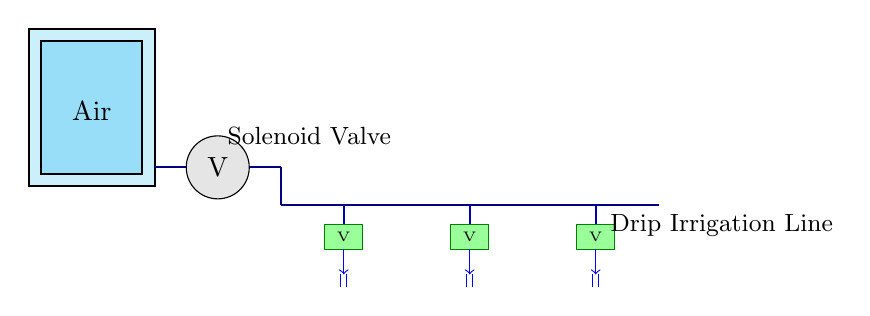
\begin{tikzpicture}[scale=0.8]
    % Ember/wadah air
    \draw[thick, fill=cyan!20] (0,0) rectangle (2,2.5);
    \draw[thick, fill=cyan!40] (0.2,0.2) rectangle (1.8,2.3);
    \node at (1,1.2) {Air};

    % Selang
    \draw[thick, blue!50!black] (2,0.3) -- (4,0.3);
    \draw[thick, blue!50!black] (4,0.3) -- (4,-0.3);
    \draw[thick, blue!50!black] (4,-0.3) -- (10,-0.3);

    % Valve
    \node[circle, draw, fill=gray!20, minimum size=0.8cm] at (3,0.3) {V};
 
    % Emitter
    \foreach \x in {5,7,9} {
        \draw[thick, blue!70!black] (\x,-0.3) -- (\x,-0.6);
        \draw[fill=green!40, draw=green!50!black] (\x-0.3,-0.6) rectangle (\x+0.3,-1.0);
        \node at (\x,-0.8) {\tiny V};
        % Drops
        \draw[blue,->] (\x,-1.0) -- (\x,-1.4);
        \draw[blue] (\x-0.05,-1.4) -- (\x-0.05,-1.6);
        \draw[blue] (\x+0.05,-1.4) -- (\x+0.05,-1.6);
    }

    % Keterangan
    \node[right] at (3,0.8) {\small Solenoid Valve};
    \node[below] at (11,-0.3) {\small Drip Irrigation Line};
\end{tikzpicture}
\caption{Skema sederhana sistem irigasi tetes}
\label{fig:drip}
\end{figure}

\section{Perbandingan Metode Penyiraman}

\begin{table}[H]
\centering
\caption{Perbandingan Metode Penyiraman Tanaman}
\label{tab:watering-methods}
\begin{longtable}{p{3cm} p{3.5cm} p{3.5cm} p{3.5cm}}
\toprule
\textbf{Parameter} & \textbf{Manual / Gembor} & \textbf{Sprinkler} & \textbf{Irigasi Tetes IoT} \\
\midrule
\endfirsthead
\toprule
\textbf{Parameter} & \textbf{Manual / Gembor} & \textbf{Sprinkler} & \textbf{Irigasi Tetes IoT} \\
\midrule
\endhead
\bottomrule
\endfoot
Efisiensi Air & 40-50\% & 50-70\% & 90-95\% \\
Kontrol Otomatis & Tidak & Terbatas & Ya (threshold) \\
Monitoring & Visual & Tidak & Real-time \\
Kontrol Jarak Jauh & Tidak & Tidak & Ya (Aplikasi) \\
Biaya Operasional & Tinggi (tenaga) & Sedang & Rendah \\
Biaya Awal & Rendah & Sedang & Sedang \\
Presisi Penyiraman & Rendah & Sedang & Tinggi \\
Dampak Kesehatan Tanaman & Sedang & Daun basah & Optimal \\
Skalabilitas & Terbatas & Baik & Sangat baik \\
\bottomrule
\end{longtable}
\end{table}


% ============================================================
%  BAB III - METODE PERANCANGAN
% ============================================================
\chapter{METODE PERANCANGAN}

\section{Diagram Blok Sistem}

Diagram blok sistem secara keseluruhan menunjukkan hubungan antara komponen utama dalam sistem ANDROMEDA.

\begin{figure}[H]
\centering
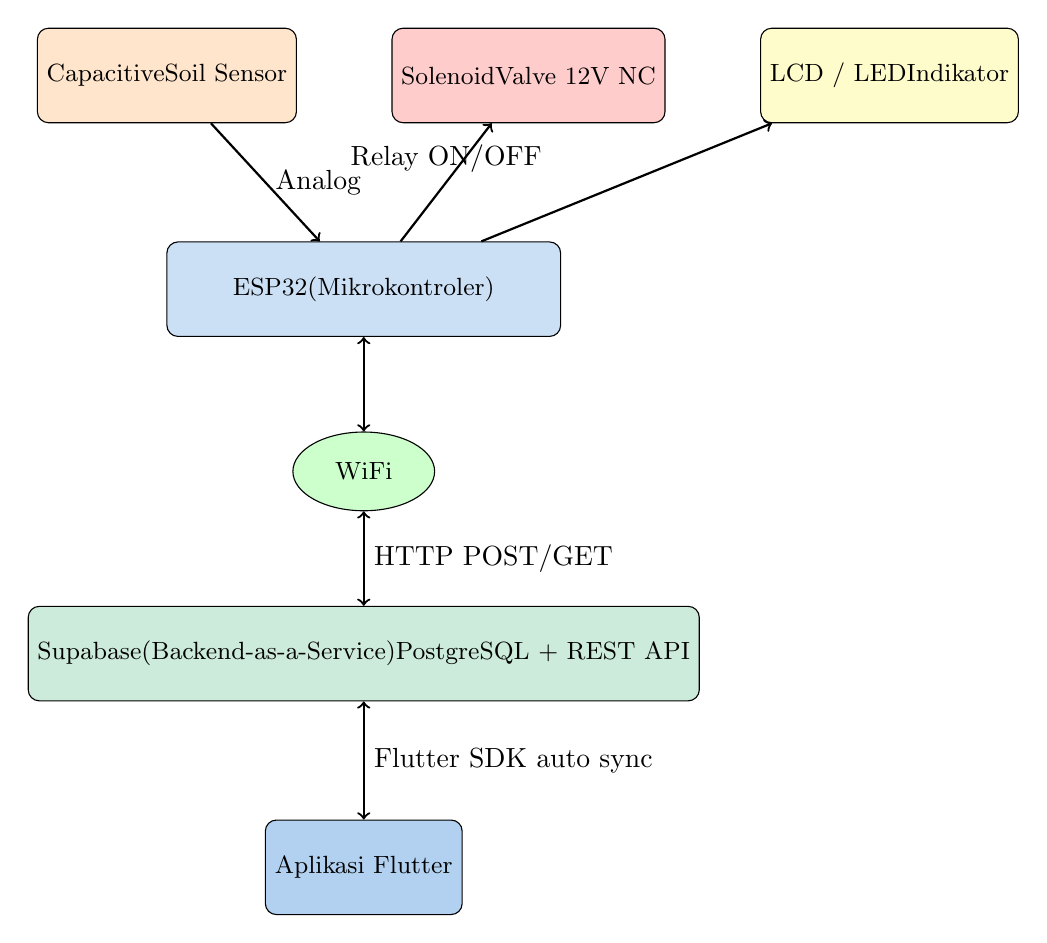
\begin{tikzpicture}[node distance=1.2cm, auto]

\tikzstyle{block} = [rectangle, rounded corners, minimum width=2.5cm, minimum height=1.2cm, text centered, draw, font=\small];
\tikzstyle{io} = [trapezium, trapezium left angle=70, trapezium right angle=110, minimum width=2cm, minimum height=1cm, text centered, draw];
\tikzstyle{cloud} = [ellipse, minimum width=1.8cm, minimum height=1cm, text centered, draw, font=\small];

% Baris 1 - Sensor/Aktuator
\node (sensor) [block, fill=orange!20] {Capacitive\\Soil Sensor};
\node (valve) [block, fill=red!20, right=of sensor] {Solenoid\\Valve 12V NC};
\node (lcd) [block, fill=yellow!20, right=of valve] {LCD / LED\\Indikator};

% Baris 2 - ESP32
\node (esp32) [block, fill=primaryblue!20, minimum width=5cm, below=1.5cm of sensor, xshift=2.5cm] {ESP32 \\ (Mikrokontroler)};

% Baris 3 - Koneksi
\node (wifi) [cloud, fill=green!20, below=1.2cm of esp32] {WiFi};

% Baris 4 - Backend (Supabase)
\node (supabase) [block, fill=accentgreen!20, minimum width=4cm, below=1.2cm of wifi] {Supabase \\ (Backend-as-a-Service) \\ PostgreSQL + REST API};
\node (android) [block, fill=primaryblue!30, below=1.5cm of supabase] {Aplikasi Flutter};

% Koneksi
\draw[->, thick] (sensor) -- node[right] {Analog} (esp32);
\draw[->, thick] (esp32) -- node[above] {Relay ON/OFF} (valve);
\draw[->, thick] (esp32) -- (lcd);
\draw[<->, thick] (esp32) -- (wifi);
\draw[<->, thick] (wifi) -- node[right] {HTTP POST/GET} (supabase);
\draw[<->, thick] (supabase) -- node[right] {Flutter SDK auto sync} (android);

\end{tikzpicture}
\caption{Diagram blok sistem ANDROMEDA}
\label{fig:block-diagram}
\end{figure}

\section{Arsitektur Sistem Lengkap}

Arsitektur sistem ANDROMEDA terdiri dari empat komponen utama yang saling terintegrasi:

\subsection{Perangkat Keras (Hardware Layer)}

\begin{itemize}
    \item \textbf{ESP32 DevKit} — Pengendali utama, membaca sensor, mengontrol relay, mengirim data via WiFi.
    \item \textbf{Capacitive Soil Sensor v1.2} — Mengukur kelembaban tanah (analog output).
    \item \textbf{Relay 1-Channel 5V} — Mengontrol solenoid valve dari sinyal digital ESP32.
    \item \textbf{Solenoid Valve 12V NC} — Membuka/menutup aliran air dari tandon (gravitasi).
    \item \textbf{Huawei B535-932 4G LTE Router} — Koneksi internet, daya 12V DC langsung dari aki.
    \item \textbf{Power Supply 12V} — Memberi daya ke ESP32, relay, dan router LTE.
    \item \textbf{Kabel Belden 3107A / UTP Cat5e} — Kabel twisted pair shielded untuk sinyal sensor ke ESP32 (\textasciitilde10--20m).
    \item \textbf{Selang Drip Irrigation} — Mendistribusikan air ke tanaman.
    \item \textbf{LED Indikator} — Status sistem (ON/OFF/Error).
\end{itemize}

\subsection{Jaringan dan Komunikasi}

\begin{itemize}
    \item \textbf{WiFi 2.4 GHz} — Koneksi internet dari ESP32 ke Huawei B535-932.
    \item \textbf{Huawei B535-932 4G LTE Router} — Menyediakan hotspot WiFi dari kartu SIM dengan paket data. Daya 12V DC langsung dari aki.
    \item \textbf{HTTP REST (Supabase API)} — ESP32 mengirim data sensor (POST) dan memeriksa perintah pending (GET).
    \item \textbf{Supabase Flutter SDK} — Aplikasi Flutter otomatis sinkron data dari Supabase tanpa perlu \textit{polling} manual.
\end{itemize}

\subsection{Backend — Supabase (Cloud, Gratis)}

Proyek ANDROMEDA menggunakan \textbf{Supabase} sebagai \textit{Backend-as-a-Service} yang menangani:

\begin{itemize}
    \item \textbf{PostgreSQL Database} — Menyimpan log sensor, konfigurasi, riwayat perintah.
    \item \textbf{REST API} — Auto-generated dari tabel database, langsung bisa dipakai ESP32.
    \item \textbf{Autentikasi} — Login pengguna aplikasi.
    \item \textbf{Realtime Subscription} — Aplikasi mendapat update data secara otomatis.
    \item \textbf{Edge Functions (opsional)} — Logika backend tambahan.
\end{itemize}

Supabase memiliki \textbf{tingkat gratis (Free Tier)} yang sangat cukup untuk proyek ANDROMEDA: 500 MB database, 2 GB bandwidth, dan \textbf{Rp 0 per bulan}. Tidak perlu menyewa VPS, tidak perlu setup server, dan tidak perlu maintenance infrastruktur.

\section{Perbandingan Perangkat Koneksi Internet untuk IoT}

Pemilihan perangkat koneksi internet merupakan faktor krusial dalam sistem IoT yang beroperasi di lokasi terpencil tanpa akses WiFi rumahan. Terdapat empat opsi utama yang dipertimbangkan untuk proyek ANDROMEDA:

\subsection{Opsi 1: WiFi Rumahan (ISP)}

Menggunakan layanan \textit{Internet Service Provider} (ISP) seperti IndiHome, First Media, atau MyRepublic yang dipasang di lokasi tanam.

\begin{itemize}
    \item \textbf{Biaya awal}: Rp 250.000 -- 500.000 (instalasi)
    \item \textbf{Biaya bulanan}: \textbf{Rp 150.000 -- 300.000} ×
    \item \textbf{Daya}: 220V AC (perlu inverter jika dari aki)
    \item \textbf{Kelebihan}: Koneksi stabil, bandwidth besar
    \item \textbf{Kekurangan}: Biaya bulanan sangat tinggi, instalasi permanen, tidak cocok untuk lokasi sawah/ladang
\end{itemize}

\subsection{Opsi 2: Pocket Mifi (Huawei E5577Cs-321)}

Modem WiFi portable dengan baterai built-in, menggunakan kartu SIM.

\begin{itemize}
    \item \textbf{Biaya awal}: Rp 250.000 -- 350.000
    \item \textbf{Biaya bulanan}: \textbf{Rp 15.000 -- 30.000} ✅
    \item \textbf{Daya}: 5V USB (baterai built-in 1500 mAh)
    \item \textbf{Kelebihan}: Murah, portabel
    \item \textbf{Kekurangan}: \textbf{Baterai cepat ngembung} jika dicharge 24/7 nonstop, tidak bisa pasang antena eksternal, WiFi jangkauan terbatas, tidak cocok untuk pemakaian permanen
\end{itemize}

\subsection{Opsi 3: USB Modem (Huawei E3372h)}

Modem 4G USB yang colok ke port USB, bisa dipasang antena eksternal.

\begin{itemize}
    \item \textbf{Biaya awal}: Rp 200.000 -- 300.000
    \item \textbf{Biaya bulanan}: \textbf{Rp 15.000 -- 30.000} ✅
    \item \textbf{Daya}: 5V USB (0.5A)
    \item \textbf{Kelebihan}: Murah, bisa antena eksternal, konsumsi daya rendah
    \item \textbf{Kekurangan}: \textbf{Butuh router tambahan} untuk jadi WiFi hotspot, konfigurasi lebih kompleks
\end{itemize}

\subsection{Opsi 4: 4G LTE Router (Huawei B535-932) — 🔥 REKOMENDASI}

Router 4G lengkap dengan WiFi, port LAN, dan dukungan antena eksternal.

\begin{itemize}
    \item \textbf{Biaya awal}: Rp 400.000 -- 500.000
    \item \textbf{Biaya bulanan}: \textbf{Rp 15.000 -- 30.000} ✅
    \item \textbf{Daya}: \textbf{12V DC langsung} (cocok dengan aki 12V)
    \item \textbf{Kelebihan}: \textbf{Colok langsung ke aki} (tanpa inverter/adaptor), dual-band WiFi 2.4+5 GHz, bisa pasang antena outdoor, stabil 24/7, tanpa baterai (tidak ngembung)
    \item \textbf{Kekurangan}: Harga awal lebih tinggi, ukuran lebih besar
\end{itemize}

\subsection{Tabel Perbandingan Lengkap}

\begin{table}[H]
\centering
\caption{Perbandingan perangkat koneksi internet untuk sistem IoT}
\label{tab:internet-compare}
\begin{tabularx}{\textwidth}{X c c c c}
\toprule
\textbf{Parameter} & \textbf{WiFi ISP} & \textbf{Mifi Pocket} & \textbf{USB Modem} & \textbf{LTE Router} \\
 & \textbf{Rumahan} & \textbf{(E5577)} & \textbf{(E3372)} & \textbf{(B535)} \\
\midrule
Harga Awal & Rp 250-500rb & Rp 250-350rb & Rp 200-300rb & \textbf{Rp 400-500rb} \\
Biaya Bulanan & \textbf{Rp 150-300rb} × & Rp 15-30rb ✅ & Rp 15-30rb ✅ & \textbf{Rp 15-30rb} ✅ \\
Daya & 220V AC & 5V USB & 5V USB & \textbf{12V DC langsung} 🔥 \\
Cocok Aki 12V? & × (butuh inverter) & ⚠️ (butuh stepdown) & ⚠️ (butuh stepdown) & \textbf{✅ Langsung colok} \\
Antena Outdoor? & Tidak & Tidak & ✅ Bisa & \textbf{✅ Bisa} \\
Pemakaian 24/7? & ✅ Stabil & × Baterai ngembung & ✅ Stabil & \textbf{✅ Stabil} \\
Koneksi WiFi & ✅ Built-in & ✅ Built-in & × Butuh router & \textbf{✅ Built-in} \\
Maturity & Sangat cocok & Kurang cocok & Cukup & \textbf{Sangat cocok} 🔥 \\
\bottomrule
\end{tabularx}
\end{table}

\subsection{Keputusan: Huawei B535-932}

\begin{figure}[H]
\centering
\begin{tikzpicture}[node distance=0.8cm]
\tikzstyle{item} = [rectangle, rounded corners, minimum width=10cm, minimum height=0.7cm, text centered, font=\small];
\tikzstyle{yes} = [fill=green!20, draw=green!50!black];
\tikzstyle{no} = [fill=red!20, draw=red!50!black];

\node (judul) [rectangle, rounded corners, fill=primaryblue!20, draw=primaryblue, minimum width=10cm, minimum height=1cm, font=\bfseries] {\large Mengapa Huawei B535-932?};

\node (aki) [yes, below=0.3cm of judul] {✅ Colok langsung ke aki 12V — tanpa inverter, tanpa adaptor};
\node (solar) [yes, below=0.1cm of aki] {✅ Daya 12W saja — aki 100Ah + panel 300Wp lebih dari cukup};
\node (outdoor) [yes, below=0.1cm of solar] {✅ Bisa pasang antena outdoor — sinyal kuat di lokasi terpencil};
\node (stabil) [yes, below=0.1cm of outdoor] {✅ Stabil 24/7 nonstop — tanpa baterai, tanpa khawatir ngembung};
\node (wifi) [yes, below=0.1cm of stabil] {✅ Dual-band WiFi — jangkauan luas sampai ke area tanam};
\node (murah) [yes, below=0.1cm of wifi] {✅ Cukup paket data Rp 15.000/bulan — irit dibanding WiFi ISP 150rb};
\node (sekali) [yes, below=0.1cm of murah] {✅ Investasi sekali Rp 400-500rb — lifetime};
\end{tikzpicture}
\caption{Alasan pemilihan Huawei B535-932 sebagai perangkat koneksi internet}
\label{fig:b535-reason}
\end{figure}

\textbf{Keputusan:} Proyek ANDROMEDA menggunakan \textbf{Huawei B535-932 4G LTE Router} karena:
\begin{enumerate}
    \item \textbf{Daya 12V DC} — langsung colok ke aki 100Ah tanpa perlu inverter atau adaptor tambahan, menghemat daya dan mengurangi titik kegagalan.
    \item \textbf{Biaya bulanan rendah} — cukup paket data Rp 15.000--30.000/bulan, jauh lebih hemat dibanding WiFi rumahan (Rp 150.000--300.000/bulan).
    \item \textbf{Stabil 24/7} — tanpa baterai built-in yang bisa ngembung, cocok untuk pemakaian nonstop di lokasi tanam.
    \item \textbf{Antena eksternal} — bisa dipasang antena outdoor untuk memperkuat sinyal 4G di lokasi terpencil.
    \item \textbf{WiFi dual-band} — memberikan jangkauan WiFi yang luas untuk ESP32 dan perangkat lain di area tanam.
\end{enumerate}

Dengan aki 100Ah dan solar panel 300Wp yang tersedia, konsumsi daya B535 (12W) sangat kecil — aki dapat bertahan sekitar 100 jam tanpa sinar matahari, dan panel 300Wp akan mengisi ulang aki dalam waktu 3-4 jam. Sistem kelistrikan lebih dari cukup untuk menjalankan router 24/7 beserta ESP32 dan solenoid valve.

\subsection{Aplikasi Flutter}

\begin{itemize}
    \item \textbf{Dashboard} — Menampilkan kelembaban terkini, status valve.
    \item \textbf{Kontrol Manual} — Tombol BUKA/TUTUP solenoid valve.
    \item \textbf{Mode Otomatis} — Sistem menyiram berdasarkan threshold.
    \item \textbf{Pengaturan Threshold} — Atur batas kering dan basah.
    \item \textbf{Log Historis} — Grafik kelembaban harian/mingguan.
    \item \textbf{Notifikasi} — Alert saat kelembaban kritis.
\end{itemize}

\par
Berikut adalah arsitektur sistem secara detail:

\begin{figure}[H]
\centering
\begin{tikzpicture}[
    node distance=1.5cm,
    box/.style={rectangle, rounded corners, minimum width=3.5cm, minimum height=1.0cm, text centered, draw, font=\small},
    server/.style={rectangle, rounded corners, minimum width=4cm, minimum height=0.8cm, text centered, draw, fill=blue!10},
    iot/.style={rectangle, rounded corners, minimum width=3cm, minimum height=0.8cm, text centered, draw, fill=green!10}
]

% Box besar - Hardware
\node (hardware) [box, fill=green!15, minimum width=6cm, minimum height=3.5cm, label={[font=\bfseries]above:{\large HARDWARE}}] {};
\node (esp) [iot, below=0.2cm of hardware.north] {ESP32 DevKit};
\node (sensor) [iot, below=0.1cm of esp] {Capacitive Soil Sensor};
\node (relay) [iot, below=0.1cm of sensor] {Relay 1ch};
\node (valve) [iot, below=0.1cm of relay] {Solenoid Valve\\12V NC + Drip};

% Box besar - Supabase Cloud
\node (supabase) [box, fill=blue!10, minimum width=5.5cm, minimum height=3.0cm, right=2cm of hardware, label={[font=\bfseries]above:{\\large SUPABASE (CLOUD, GRATIS)}}] {};
\node (db) [server, below=0.2cm of supabase.north] {PostgreSQL Database};
\node (api) [server, below=0.1cm of db] {Auto-generated REST API};
\node (auth) [server, below=0.1cm of api] {Authentication};
\node (rt) [server, below=0.1cm of auth] {Realtime Subscription};

% Flutter App
\node (android) [box, fill=orange!15, minimum width=4.5cm, minimum height=1.2cm, below=2cm of supabase, label={[font=\\bfseries]above:{\\large FLUTTER APP}}] {};
\node at (android) {Monitor \\& Control \\ (Supabase Flutter SDK)};

% Koneksi
\draw[<->, thick, primaryblue] (esp.east) -- node[above] {HTTP POST/GET} (api.west);
\draw[<->, thick, primaryblue] (api.east) -- ++(1,0) -- ++(0,-3.0) -- node[above] {Flutter SDK auto sync} (android.east);
\draw[<->, thick] (db.south) -- (api.north);
\draw[<->, thick] (api.south) -- (rt.north);
\draw[<->, thick] (auth.south) -- (rt.north);

% Internet cloud
\node[cloud, draw, fill=gray!10, minimum width=1.2cm, minimum height=0.8cm] at ($(hardware.east)!0.5!(supabase.west)$) {\\small Internet};
\draw[dashed] ($(hardware.east)+(0,-0.2)$) -- ($(hardware.east)+(0,1.0)$);
\draw[dashed] ($(supabase.west)+(-0,2.5)$) -- ($(supabase.west)+(-0,0.5)$);

\end{tikzpicture}
\caption{Arsitektur sistem ANDROMEDA secara keseluruhan}
\label{fig:full-arch}
\end{figure}

\section{Flowchart Sistem}

\subsection{Alur Sistem Utama}

\begin{figure}[H]
\centering
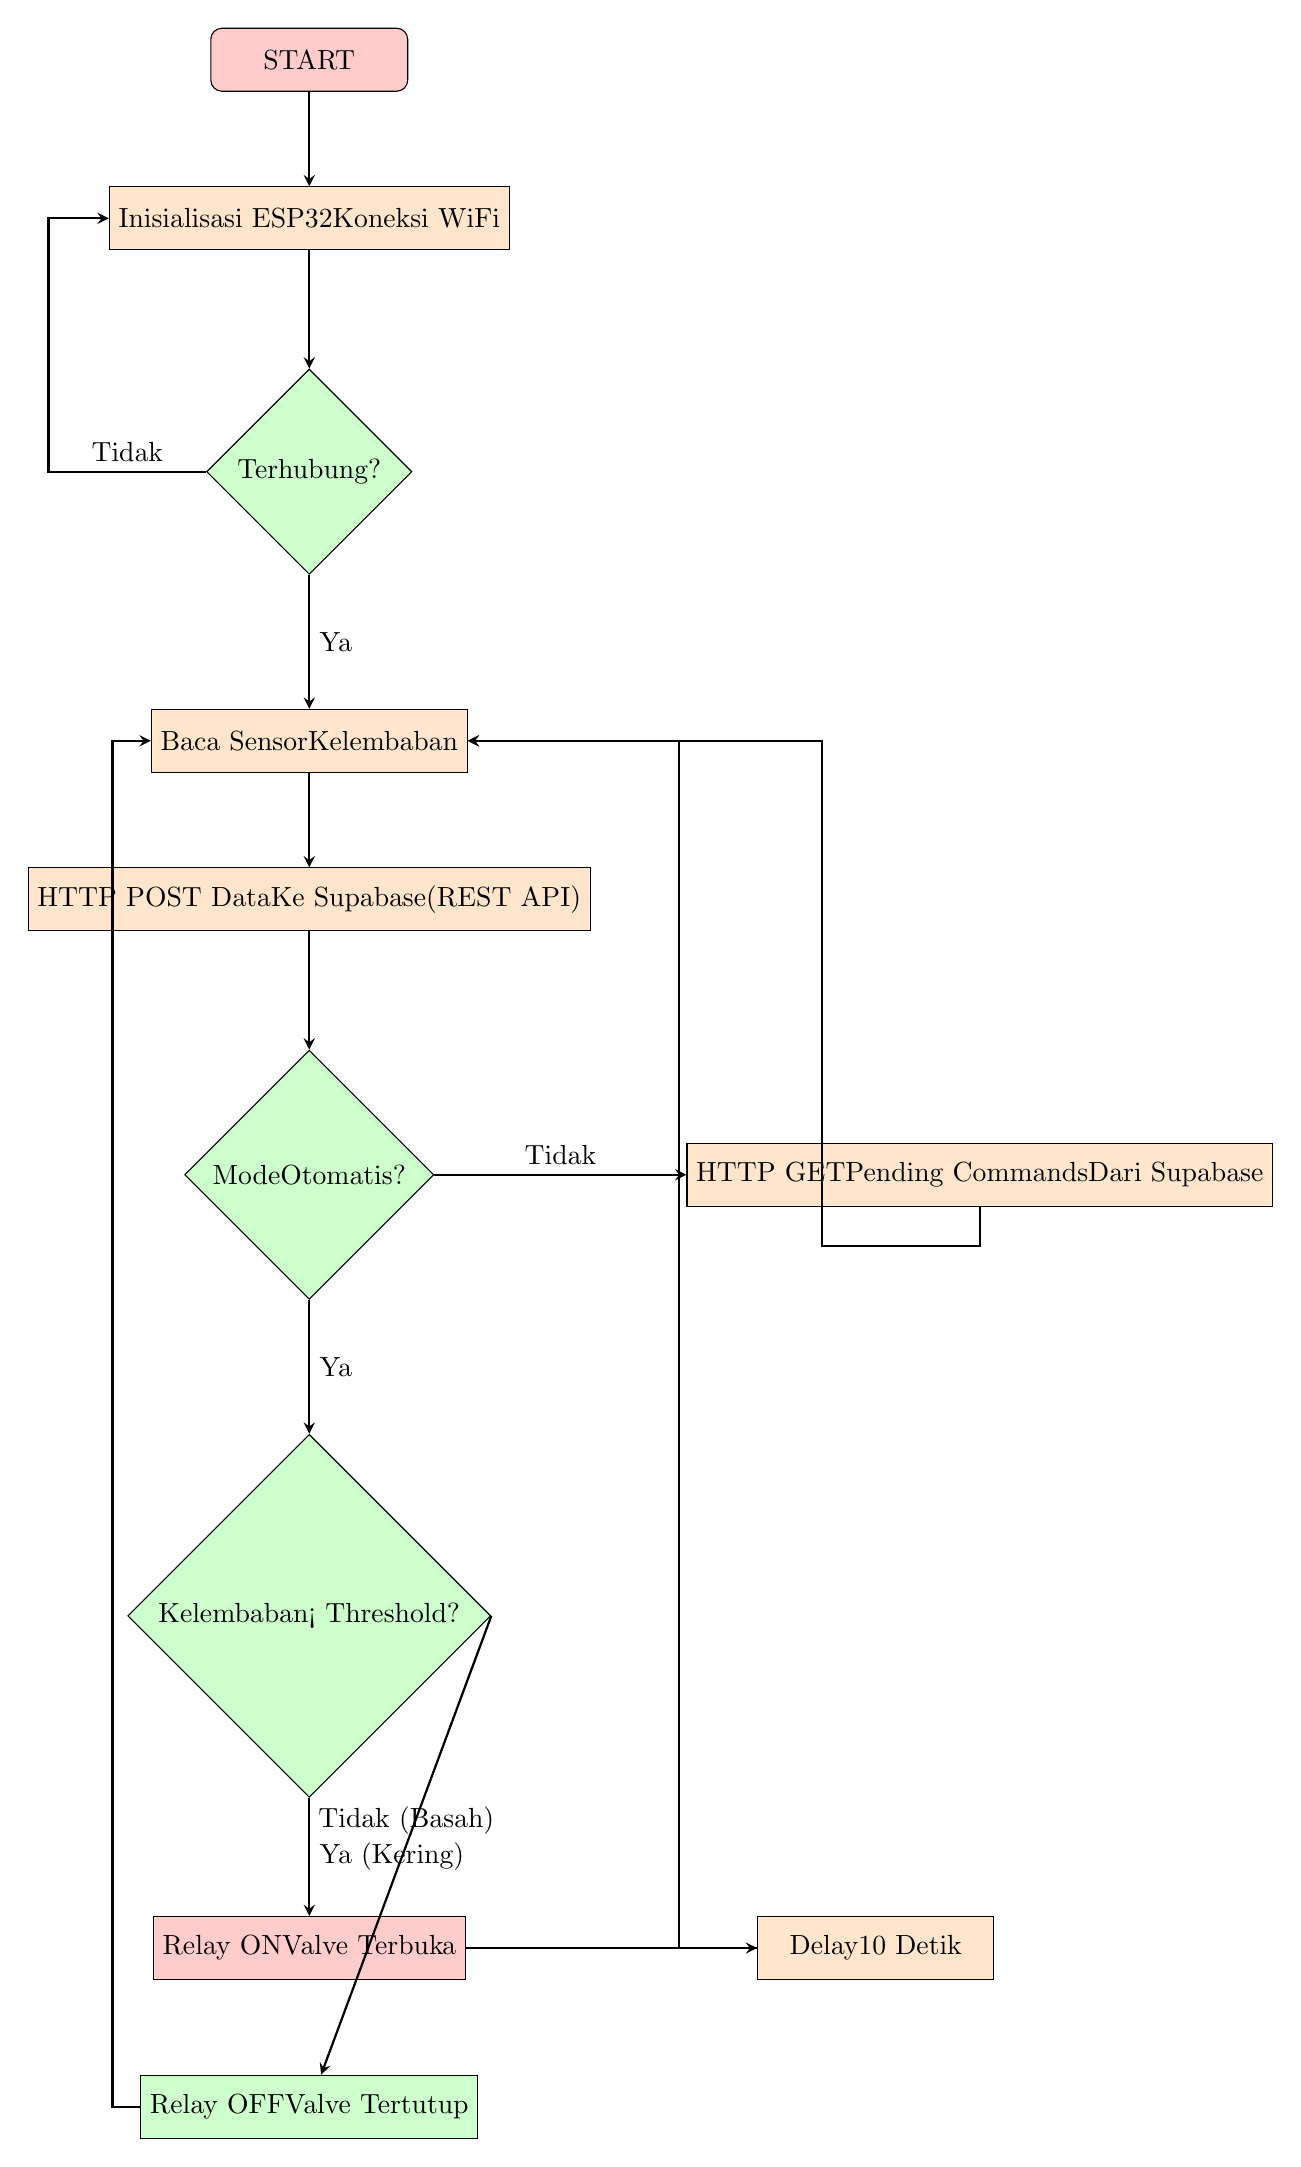
\begin{tikzpicture}[
    node distance=1.2cm,
    startstop/.style={rectangle, rounded corners, minimum width=2.5cm, minimum height=0.8cm, text centered, draw, fill=red!20},
    io/.style={trapezium, trapezium left angle=70, trapezium right angle=110, minimum width=2cm, minimum height=0.8cm, text centered, draw, fill=blue!20},
    process/.style={rectangle, minimum width=3cm, minimum height=0.8cm, text centered, draw, fill=orange!20},
    decision/.style={diamond, minimum width=2.5cm, minimum height=1.5cm, text centered, draw, fill=green!20},
    arrow/.style={thick, ->, >=stealth}
]

\node (start) [startstop] {START};
\node (init) [process, below=of start] {Inisialisasi ESP32\\Koneksi WiFi};
\node (check) [decision, below=of init, yshift=-0.3cm] {Terhubung?};
\node (read) [process, below=of check, yshift=-0.5cm] {Baca Sensor\\Kelembaban};
\node (send) [process, below=of read] {HTTP POST Data\\Ke Supabase\\ (REST API)};
\node (mode) [decision, below=of send, yshift=-0.3cm] {Mode\\Otomatis?};
\node (manual) [process, right=of mode, xshift=2cm] {HTTP GET\\Pending Commands\\Dari Supabase};
\node (dry) [decision, below=of mode, yshift=-0.5cm] {Kelembaban\\< Threshold?};
\node (pump_on) [process, below=of dry, yshift=-0.3cm, fill=red!20] {Relay ON\\Valve Terbuka};
\node (pump_off) [process, below=of pump_on, fill=green!20] {Relay OFF\\Valve Tertutup};
\node (wait) [process, right=of pump_on, xshift=2.5cm] {Delay\\10 Detik};

% Arrows
\draw[arrow] (start) -- (init);
\draw[arrow] (init) -- (check);
\draw[arrow] (check) -- node[right] {Ya} (read);
\draw[arrow] (check.west) -- node[above] {Tidak} ++(-2,0) |- (init);
\draw[arrow] (read) -- (send);
\draw[arrow] (send) -- (mode);
\draw[arrow] (mode) -- node[right] {Ya} (dry);
\draw[arrow] (mode.east) -- node[above] {Tidak} (manual);
\draw[arrow] (dry) -- node[right] {Ya (Kering)} (pump_on);
\draw[arrow] (dry.east) -- node[above] {Tidak (Basah)} (pump_off);
\draw[arrow] (pump_on) -- (wait);
\draw[arrow] (wait) -- ++(-2.5,0) |- (read);
\draw[arrow] (pump_off) -- ++(-2.5,0) |- (read);
\draw[arrow] (manual.south) -- ++(0,-0.5) -- ++(-2,0) |- (read);

\end{tikzpicture}
\caption{Flowchart sistem ANDROMEDA}
\label{fig:flowchart}
\end{figure}

\subsection{Alur Aplikasi Flutter}

\begin{figure}[H]
\centering
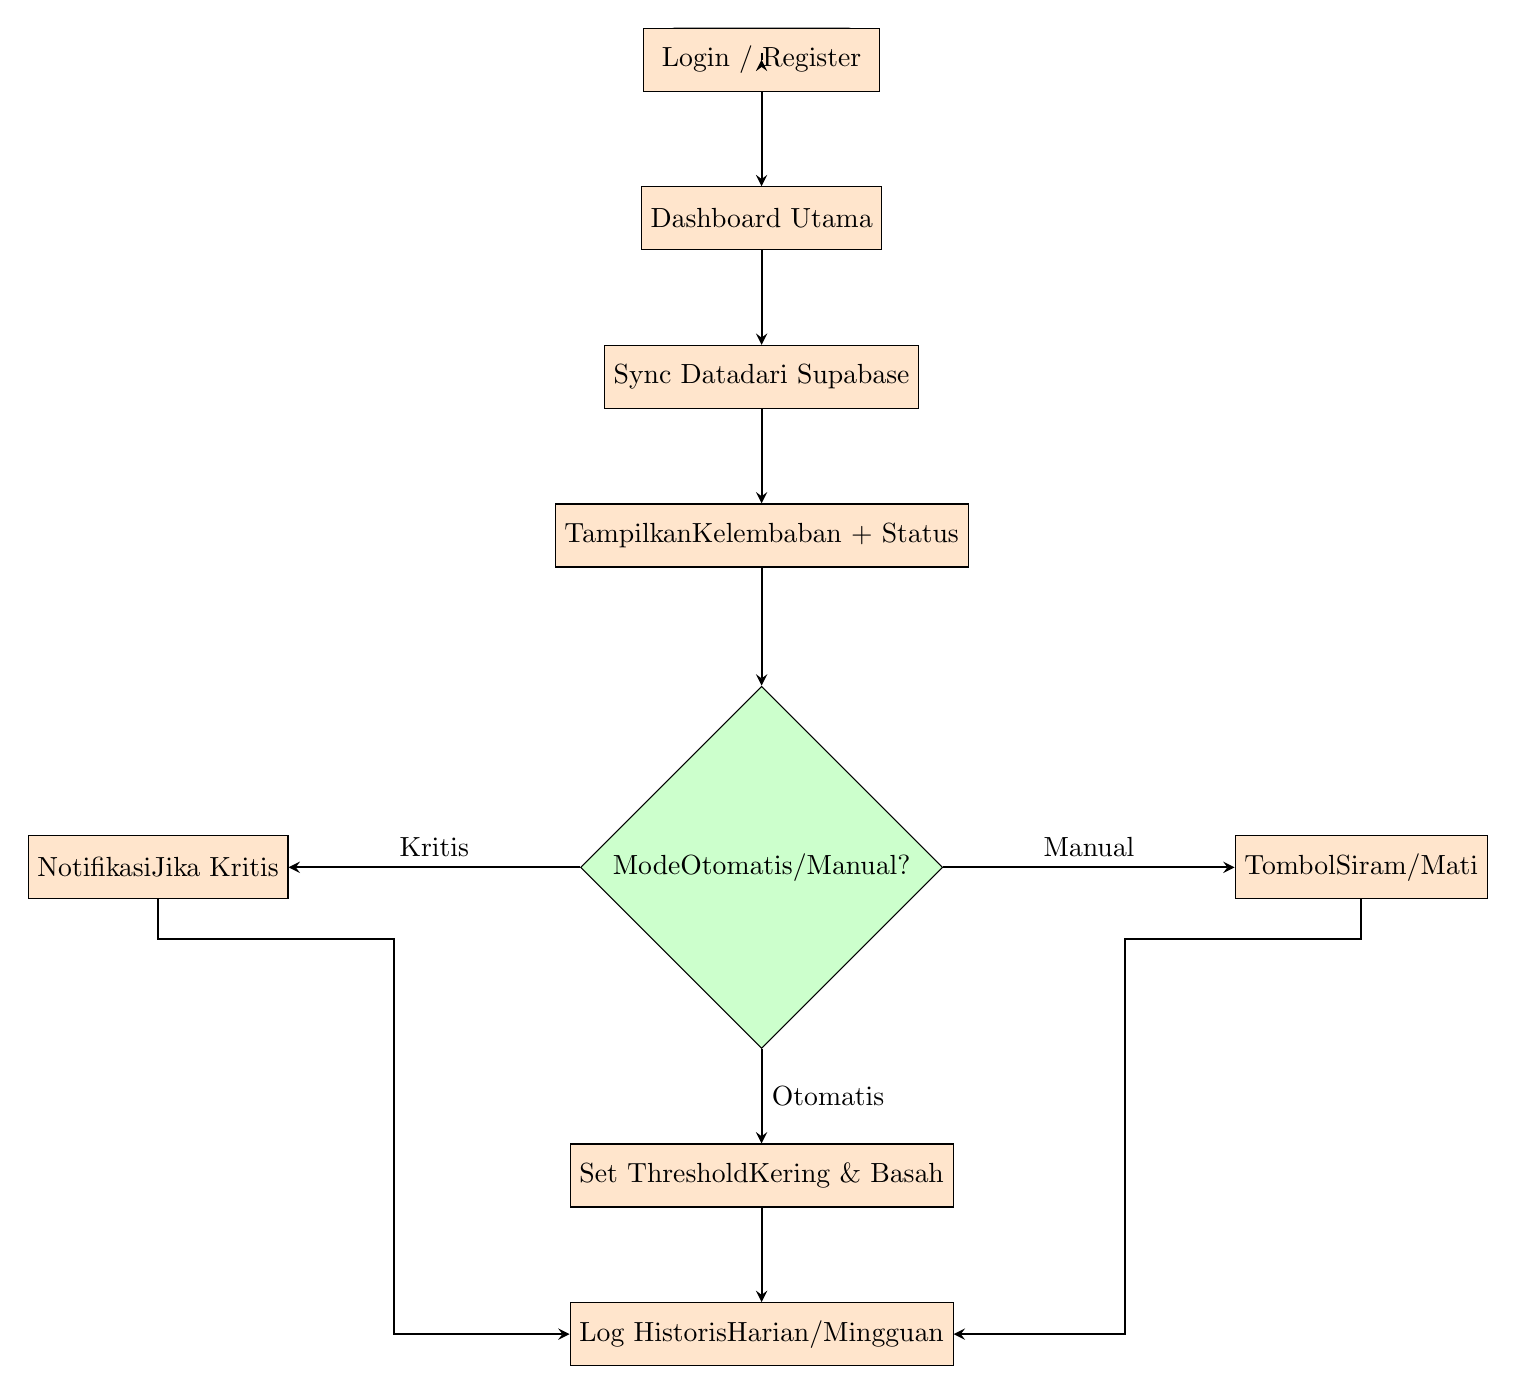
\begin{tikzpicture}[
    node distance=1.2cm,
    startstop/.style={rectangle, rounded corners, minimum width=2.5cm, minimum height=0.8cm, text centered, draw, fill=red!20},
    process/.style={rectangle, minimum width=3cm, minimum height=0.8cm, text centered, draw, fill=orange!20},
    decision/.style={diamond, minimum width=2.2cm, minimum height=1.5cm, text centered, draw, fill=green!20},
    arrow/.style={thick, ->, >=stealth}
]

\node (start) [startstop] {Buka Aplikasi};
\node (login) [process] {Login / Register};
\node (dash) [process, below=of login] {Dashboard Utama};
\node (sync) [process, below=of dash] {Sync Data\\dari Supabase};
\node (disp) [process, below=of sync] {Tampilkan\\Kelembaban + Status};
\node (mode_sel) [decision, below=of disp, yshift=-0.3cm] {Mode\\Otomatis/Manual?};
\node (btn_man) [process, right=of mode_sel, xshift=2.5cm] {Tombol\\Siram/Mati};
\node (auto_sel) [process, below=of mode_sel] {Set Threshold\\Kering \& Basah};
\node (hist) [process, below=of auto_sel] {Log Historis\\Harian/Mingguan};
\node (notif) [process, left=of mode_sel, xshift=-2.5cm] {Notifikasi\\Jika Kritis};

\draw[arrow] (start) -- (login);
\draw[arrow] (login) -- (dash);
\draw[arrow] (dash) -- (sync);
\draw[arrow] (sync) -- (disp);
\draw[arrow] (disp) -- (mode_sel);
\draw[arrow] (mode_sel.east) -- node[above] {Manual} (btn_man);
\draw[arrow] (mode_sel) -- node[right] {Otomatis} (auto_sel);
\draw[arrow] (auto_sel) -- (hist);
\draw[arrow] (mode_sel.west) -- node[above] {Kritis} (notif);
\draw[arrow] (notif.south) -- ++(0,-0.5) -- ++(3,0) |- (hist);
\draw[arrow] (btn_man.south) -- ++(0,-0.5) -- ++(-3,0) |- (hist);

\end{tikzpicture}
\caption{Flowchart aplikasi Flutter ANDROMEDA}
\label{fig:android-flow}
\end{figure}

\section{Spesifikasi Hardware Lengkap}

\begin{table}[H]
\centering
\caption{Daftar komponen hardware sistem ANDROMEDA}
\label{tab:hardware}
\begin{tabularx}{\textwidth}{c X c c}
\toprule
\textbf{No} & \textbf{Komponen} & \textbf{Qty} & \textbf{Harga} \\
\midrule
1 & ESP32 DevKit (WiFi + Bluetooth) & 1 & Rp 65.000 \\
2 & Capacitive Soil Sensor v1.2 & 1 & Rp 35.000 \\
3 & Relay Module 1 Channel 5V & 1 & Rp 12.000 \\
4 & Solenoid Valve 12V NC & 1 & Rp 50.000 \\
5 & Power Supply 12V (dari aki via step-down) & 1 & Rp 25.000 \\
7 & Selang Drip Irrigation 10m & 1 & Rp 30.000 \\
8 & Dripper / Emitter (10 pcs) & 1 pack & Rp 15.000 \\
9 & Kabel Jumper (M-M, M-F, F-F) & 1 set & Rp 15.000 \\
10 & Project Box (kotak panel) & 1 & Rp 20.000 \\
11 & LED Indikator + Resistor & 3 & Rp 5.000 \\
12 & PCB Prototype / Breadboard & 1 & Rp 10.000 \\
13 & Konektor dan terminal & 1 set & Rp 10.000 \\
\midrule
\multicolumn{3}{r}{\textbf{Total Hardware (1 titik)}} & \textbf{Rp 292.000} \\
\multicolumn{3}{r}{} & \\
\multicolumn{3}{r}{\textbf{+ LTE Router (sekali beli)}} & \textbf{Rp 450.000} \\
\multicolumn{3}{r}{\textbf{Total Awal}} & \textbf{Rp 742.000} \\
\bottomrule
\end{tabularx}
\end{table}

\section{Spesifikasi Software}

\begin{table}[H]
\centering
\caption{Software yang digunakan dalam pengembangan sistem ANDROMEDA}
\label{tab:software}
\begin{tabularx}{\textwidth}{c X X}
\toprule
\textbf{No} & \textbf{Software / Platform} & \textbf{Fungsi} \\
\midrule
1 & Arduino IDE / PlatformIO & Programming ESP32 (C/C++) \\
2 & \textbf{Supabase (Backend-as-a-Service)} & Database, REST API, Auth — \textbf{gratis} \\
3 & Flutter SDK (Dart) & Pengembangan aplikasi lintas platform \\
4 & Supabase Flutter SDK & Sinkronisasi data real-time \\
5 & HTTPClient Library (ESP32) & HTTP POST/GET ke Supabase REST API \\
6 & ArduinoJson & Parsing JSON dari Supabase \\
7 & fl\_chart & Grafik data historis \\
\bottomrule
\end{tabularx}
\end{table}

\section{Rancangan Rangkaian}

\subsection{Skematik ESP32 ke Sensor dan Relay}

\begin{figure}[H]
\centering
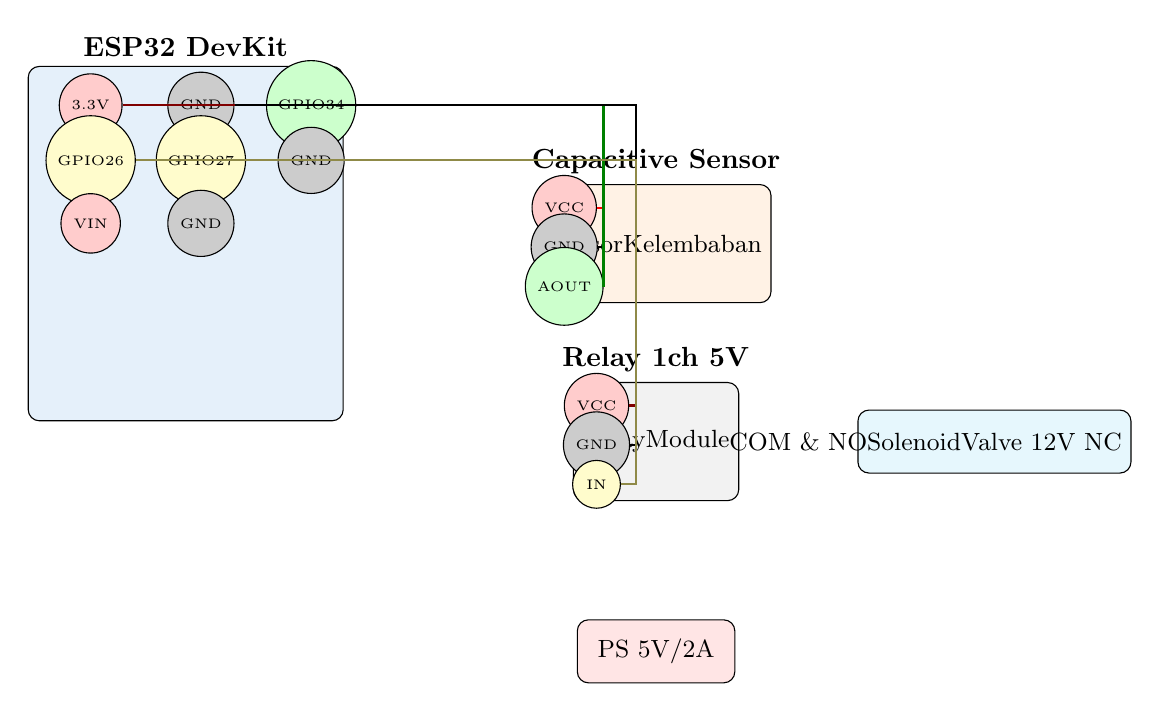
\begin{tikzpicture}[
    component/.style={rectangle, rounded corners, minimum width=2.5cm, minimum height=0.8cm, text centered, draw, font=\small},
    pin/.style={circle, minimum width=0.4cm, draw, font=\tiny}
]

% ESP32
\node (esp) [component, fill=primaryblue!10, minimum width=4cm, minimum height=4.5cm] {};
\node[above] at (esp.north) {\textbf{ESP32 DevKit}};

% Pin ESP32
\node (3v3) [pin, fill=red!20] at ($(esp.north west)+(0.8,-0.5)$) {3.3V};
\node (gnd1) [pin, fill=black!20] at ($(esp.north west)+(2.2,-0.5)$) {GND};
\node (gpio34) [pin, fill=green!20] at ($(esp.north west)+(3.6,-0.5)$) {GPIO34};
\node (gpio26) [pin, fill=yellow!20] at ($(esp.north west)+(0.8,-1.2)$) {GPIO26};
\node (gpio27) [pin, fill=yellow!20] at ($(esp.north west)+(2.2,-1.2)$) {GPIO27};
\node (gnd2) [pin, fill=black!20] at ($(esp.north west)+(3.6,-1.2)$) {GND};
\node (vin) [pin, fill=red!20] at ($(esp.north west)+(0.8,-2.0)$) {VIN};
\node (gnd3) [pin, fill=black!20] at ($(esp.north west)+(2.2,-2.0)$) {GND};

% Sensor
\node (sensor) [component, fill=orange!10, minimum width=2cm, minimum height=1.5cm, right=2.5cm of esp] {Sensor\\Kelembaban};
\node[above] at (sensor.north) {\textbf{Capacitive Sensor}};
\node (svcc) [pin, fill=red!20] at ($(sensor.north west)+(0.3,-0.3)$) {VCC};
\node (sgnd) [pin, fill=black!20] at ($(sensor.north west)+(0.3,-0.8)$) {GND};
\node (sout) [pin, fill=green!20] at ($(sensor.north west)+(0.3,-1.3)$) {AOUT};

% Relay
\node (relay) [component, fill=gray!10, minimum width=2cm, minimum height=1.5cm, below=1cm of sensor] {Relay\\Module};
\node[above] at (relay.north) {\textbf{Relay 1ch 5V}};
\node (rvcc) [pin, fill=red!20] at ($(relay.north west)+(0.3,-0.3)$) {VCC};
\node (rgnd) [pin, fill=black!20] at ($(relay.north west)+(0.3,-0.8)$) {GND};
\node (rin) [pin, fill=yellow!20] at ($(relay.north west)+(0.3,-1.3)$) {IN};

% Solenoid Valve
\node (pomp) [component, fill=cyan!10, minimum width=2cm, minimum height=0.8cm, right=1.5cm of relay] {Solenoid\\Valve 12V NC};
\node at ($(relay.east)!0.5!(pomp.west)$) {\small COM \& NO};

% Power Supply
\node (ps) [component, fill=red!10, minimum width=2cm, minimum height=0.8cm, below=1.5cm of relay] {PS 5V/2A};

% Koneksi
\draw[red, thick] (svcc) -- ++(0.5,0) |- (3v3);
\draw[black, thick] (sgnd) -- ++(0.5,0) |- (gnd1);
\draw[green!50!black, thick] (sout) -- ++(0.5,0) |- (gpio34);
\draw[red!50!black, thick] (rvcc) -- ++(0.5,0) |- (3v3);
\draw[black, thick] (rgnd) -- ++(0.5,0) |- (gnd1);
\draw[yellow!50!black, thick] (rin) -- ++(0.5,0) |- (gpio26);

\end{tikzpicture}
\caption{Skematik koneksi ESP32 ke sensor dan relay}
\label{fig:schematic}
\end{figure}

\subsection{Tabel Koneksi Pin}

\begin{table}[H]
\centering
\caption{Koneksi pin ESP32 ke komponen}
\label{tab:pinout}
\begin{tabular}{c c c}
\toprule
\textbf{Pin ESP32} & \textbf{Komponen} & \textbf{Keterangan} \\
\midrule
3.3V & Capacitive Sensor VCC & Catu daya sensor \\
3.3V & Relay VCC & Catu daya relay \\
GND & Semua komponen GND & Ground bersama \\
GPIO34 (ADC) & Capacitive Sensor AOUT & Membaca sinyal analog sensor langsung \\
GPIO26 & Relay IN & Kontrol solenoid valve (HIGH = ON) \\
GPIO27 & LED Indikator & Status sistem \\
\bottomrule
\end{tabular}
\end{table}


% ============================================================
%  SECTION - TRANSMISI SINYAL SENSOR
% ============================================================
\newpage
\section{Transmisi Sinyal Sensor}

\subsection{Pertimbangan Jarak}

Berdasarkan kondisi lapangan di PDB Desa Merayan, sensor kelembaban tanah ditempatkan di lahan yang berjarak sekitar \textbf{10--20 meter} dari panel kontrol yang berisi ESP32 dan sistem kelistrikan. Untuk jarak tersebut, pendekatan yang digunakan adalah koneksi langsung menggunakan kabel \textit{twisted pair shielded} dengan pertimbangan:

\begin{enumerate}
    \item \textbf{Voltage drop minimal} --- Pada jarak 20m dengan kabel AWG24, resistansi total hanya ∼3,4$\Omega$. Dengan arus output sensor ∼5 mA, drop tegangan hanya ∼17 mV --- tidak signifikan untuk ADC 12-bit ESP32.
    \item \textbf{Noise elektromagnetik} --- Diredam dengan kabel \textit{twisted pair shielded} (Belden 3107A atau UTP Cat5e) yang meminimalkan induksi dari solenoid valve dan router LTE di sekitar.
    \item \textbf{Sederhana dan andal} --- Tidak perlu IC tambahan seperti XTR116, tidak perlu rangkaian konversi 4-20mA, tidak perlu kalibrasi khusus.
\end{enumerate}

\subsection{Solusi: Koneksi Langsung via Kabel Shielded}

Capacitive Soil Sensor v1.2 dihubungkan langsung ke ESP32 melalui kabel \textit{twisted pair shielded} sebagai berikut:

\begin{itemize}
    \item \textbf{VCC Sensor} $\to$ 3.3V ESP32 (via kabel twisted pair)
    \item \textbf{GND Sensor} $\to$ GND ESP32 (via kabel twisted pair)
    \item \textbf{AOUT Sensor} $\to$ GPIO34 (ADC) ESP32 (via kabel twisted pair)
    \item Kapasitor 100nF dipasang di pin ADC ESP32 sebagai filter \textit{decoupling} untuk meredam noise frekuensi tinggi.
\end{itemize}

\begin{figure}[H]
\centering
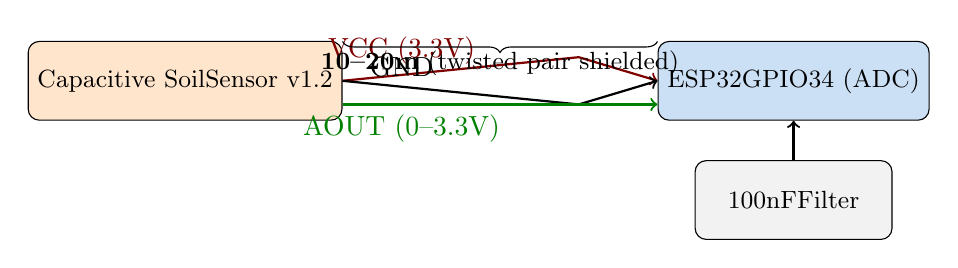
\begin{tikzpicture}[
    comp/.style={rectangle, rounded corners, minimum width=2.5cm, minimum height=1cm, text centered, draw, font=\small}
]

% Sensor
\node (sensor) [comp, fill=orange!20] {Capacitive Soil \\ Sensor v1.2};
\node (esp) [comp, fill=primaryblue!20, right=4cm of sensor] {ESP32 \\ GPIO34 (ADC)};
\node (cap) [comp, fill=gray!10, below=0.5cm of esp] {100nF \\ Filter};

% Koneksi
\draw[->, thick, red!50!black] (sensor.east) -- node[above] {VCC (3.3V)} ++(1.5,0.15) -- ++(1.5,0.15) -- (esp.west);
\draw[->, thick, black] (sensor.east) -- node[above] {GND} ++(1.5,-0.15) -- ++(1.5,-0.15) -- (esp.west);
\draw[->, thick, green!50!black] ([yshift=-0.3cm]sensor.east) -- node[below] {AOUT (0--3.3V)} ++(1.5,0) -- ++(1.5,0) -- ([yshift=-0.3cm]esp.west);
\draw[->, thick] (cap.north) -- (esp.south);

% Anotasi kabel
\draw[decorate, decoration={brace, amplitude=4pt, mirror}]
    ([yshift=0.5cm]sensor.east) -- node[below, font=\small] {\textbf{10--20m} (twisted pair shielded)} ([yshift=0.5cm]esp.west);

\end{tikzpicture}
\caption{Koneksi langsung sensor ke ESP32 via kabel twisted pair shielded}
\label{fig:direct-wiring}
\end{figure}

\subsection{Rekomendasi Kabel}

\begin{table}[H]
\centering
\caption{Rekomendasi kabel untuk koneksi sensor}
\label{tab:cable-rec}
\begin{tabularx}{\textwidth}{l X c c}
\toprule
\textbf{Jenis Kabel} & \textbf{Keunggulan} & \textbf{Harga/m} & \textbf{Kebutuhan} \\
\midrule
\textbf{Belden 3107A} & 2-pair twisted + foil shield, noise immunity tinggi & Rp 10.000--12.000 & 20m \\
Alternatif: UTP Cat5e & 4-pair twisted, mudah didapat, murah & Rp 3.000--5.000 & 20m \\
\bottomrule
\end{tabularx}
\end{table}

Kabel Belden 3107A direkomendasikan untuk instalasi permanen di luar ruangan karena konstruksinya yang lebih kokoh dan shielded yang lebih baik. Sebagai alternatif hemat, UTP Cat5e juga cukup memadai untuk jarak 10--20m.


% ============================================================
%  BAB IV - RENCANA IMPLEMENTASI
% ============================================================
\chapter{RENCANA IMPLEMENTASI}

\section{Tahapan Pengembangan}

Proyek ANDROMEDA dikembangkan dalam empat tahap utama:

\begin{enumerate}
    \item \textbf{Tahap 1: Perakitan Hardware}
    \begin{itemize}
        \item Menyiapkan dan menguji komponen (ESP32, sensor, relay, solenoid valve).
        \item Merangkai komponen sesuai skematik.
        \item Uji coba pembacaan sensor dan aktuasi valve.
    \end{itemize}
    
    \item \textbf{Tahap 2: Firmware ESP32}
    \begin{itemize}
        \item Programming ESP32 dengan Arduino IDE/PlatformIO.
        \item Implementasi pembacaan sensor ADC.
        \item Implementasi koneksi WiFi dan HTTP client.
        \item Logika kontrol otomatis (threshold-based).
        \item HTTP POST data sensor ke Supabase REST API.
        \item HTTP GET perintah pending dari Supabase.
        \item Mode deep sleep untuk efisiensi daya.
    \end{itemize}
    
    \item \textbf{Tahap 3: Setup Supabase (Backend)}
    \begin{itemize}
        \item Membuat project di Supabase (\textbf{Free Tier} — Rp 0/bulan).
        \item Membuat tabel database: \texttt{sensor\_readings}, \texttt{pending\_commands}, \texttt{system\_config}.
        \item Mengaktifkan REST API (auto-generated, langsung bisa dipakai).
        \item Setup Authentication untuk login aplikasi Flutter.
        \item Uji coba HTTP POST dari ESP32 dan HTTP GET dari Flutter.
    \end{itemize}
    
    \item \textbf{Tahap 4: Aplikasi Flutter}
    \begin{itemize}
        \item UI/UX Design (Dashboard, Control, Settings) menggunakan Flutter (Dart).
        \item Integrasi Supabase Flutter SDK (auto sync data real-time).
        \item Autentikasi login pengguna.
        \item Grafik data historis menggunakan fl\_chart.
        \item Notifikasi push.
    \end{itemize}
\end{enumerate}

\section{Tabel Database Supabase}

\begin{table}[H]
\centering
\caption{Daftar tabel database Supabase yang digunakan}
\label{tab:supabase-tables}
\begin{tabularx}{\textwidth}{c X X X}
\toprule
\textbf{No} & \textbf{Tabel} & \textbf{Fungsi} & \textbf{Diakses Oleh} \\
\midrule
1 & \texttt{sensor\_readings} & Menyimpan log kelembaban + timestamp & ESP32 (POST), Flutter (GET) \\
2 & \texttt{pending\_commands} & Antrian perintah dari Flutter ke ESP32 & Flutter (POST), ESP32 (GET) \\
3 & \texttt{system\_config} & Threshold, mode Auto/Manual & Flutter (RW), ESP32 (GET) \\
4 & \texttt{users} & Data login pengguna aplikasi & Flutter (Auth) \\
\bottomrule
\end{tabularx}
\end{table}

\section{Rencana Pengujian}

\begin{table}[H]
\centering
\caption{Rencana pengujian sistem}
\label{tab:testing}
\begin{tabularx}{\textwidth}{c X X}
\toprule
\textbf{No} & \textbf{Skenario} & \textbf{Indikator Sukses} \\
\midrule
1 & Sensor membaca tanah kering & Output ADC $>$ 2700 (kering) \\
2 & Sensor membaca tanah basah & Output ADC $<$ 1500 (basah) \\
3 & ESP32 konek WiFi & LED biru menyala, log sukses \\
4 & ESP32 HTTP POST ke Supabase & Data masuk di tabel sensor\_readings \\
5 & Flutter baca dari Supabase & Dashboard menampilkan data \\
6 & Threshold kering tercapai & Valve otomatis terbuka (ON) \\
7 & Threshold basah tercapai & Valve otomatis tertutup (OFF) \\
8 & Flutter kirim perintah Siram & Entry muncul di pending\_commands \\
9 & ESP32 ambil perintah pending & Valve menyala sesuai perintah \\
10 & Data historis tersimpan & Tabel sensor\_readings terisi \\
\bottomrule
\end{tabularx}
\end{table}


% ============================================================
%  SECTION - RINCIAN ALAT DAN BAHAN (BILL OF MATERIALS)
% ============================================================
\newpage
\section{Rincian Alat dan Bahan (Bill of Materials)}

Berikut adalah daftar lengkap seluruh komponen yang dibutuhkan untuk implementasi sistem ANDROMEDA beserta estimasi harga dan tautan pembelian di \textit{Shopee}.


\subsection{Tabel Bill of Materials (BOM)}

\begin{table}[H]
\centering
\caption{Bill of Materials — Sistem ANDROMEDA}
\label{tab:bom}
\begin{tabularx}{\textwidth}{c X c c c}
\toprule
\textbf{No} & \textbf{Komponen} & \textbf{Qty} & \textbf{Estimasi Harga} & \textbf{Link Shopee} \\
\midrule
1 & ESP32 DevKit Board 30 Pin & 1 & Rp 45.000 -- 60.000 & \href{https://shopee.co.id/search?keyword=ESP32+DevKit+Board+30+pin}{Cari di Shopee} \\
2 & Capacitive Soil Sensor v1.2 & 1 & Rp 15.000 -- 25.000 & \href{https://shopee.co.id/search?keyword=capacitive+soil+sensor+arduino}{Cari di Shopee} \\
3 & Relay Module 1-Channel 5V Optocoupler & 1 & Rp 8.000 -- 15.000 & \href{https://shopee.co.id/search?keyword=relay+1+channel+5V+optocoupler}{Cari di Shopee} \\
4 & Solenoid Valve 12V NC 1/2 inch & 1 & Rp 50.000 -- 80.000 & \href{https://shopee.co.id/search?keyword=solenoid+valve+12V+NC+1+2+inch+air}{Cari di Shopee} \\
5 & LED Indikator 5mm (biru/merah) & 2 & Rp 1.000 -- 2.000 & \href{https://shopee.co.id/search?keyword=LED+5mm+indikator+merah+biru}{Cari di Shopee} \\
6 & Resistor 220$\Omega$ (untuk LED) & 2 & Rp 500 -- 1.000 & \href{https://shopee.co.id/search?keyword=resistor+220+ohm}{Cari di Shopee} \\
7 & Huawei B535-932 4G LTE Router & 1 & Rp 400.000 -- 500.000 & \href{https://shopee.co.id/search?keyword=Huawei+B535+router+4G+LTE}{Cari di Shopee} \\
8 & Power Supply 12V 2A Adaptor & 1 & Rp 25.000 -- 40.000 & \href{https://shopee.co.id/search?keyword=power+supply+12V+2A+adaptor}{Cari di Shopee} \\
9 & Aki Kering 100Ah (Yuasa NS70 or setara) & 1 & Rp 900.000 -- 1.200.000 & \href{https://shopee.co.id/search?keyword=aki+kering+100Ah+NS70}{Cari di Shopee} \\
10 & Solar Panel 300Wp Polycrystalline & 1 & Rp 1.000.000 -- 1.500.000 & \href{https://shopee.co.id/search?keyword=solar+panel+300wp+polycrystalline}{Cari di Shopee} \\
11 & Solar Charge Controller 12/24V 20A PWM & 1 & Rp 100.000 -- 150.000 & \href{https://shopee.co.id/search?keyword=solar+charge+controller+20A+PWM}{Cari di Shopee} \\
12 & Kabel Belden 3107A / UTP Cat5e (shielded) & 20m & Rp 60.000 -- 240.000 & \href{https://shopee.co.id/search?keyword=Belden+3107A+kabel+shielded}{Cari di Shopee} \\
13 & Kabel NYMHY 2×1,5mm & 10m & Rp 30.000 -- 50.000 & \href{https://shopee.co.id/search?keyword=NYMHY+2x1.5+listrik}{Cari di Shopee} \\
14 & Kabel Jumper Male-Female 20cm & 20 pcs & Rp 5.000 -- 10.000 & \href{https://shopee.co.id/search?keyword=kabel+jumper+male+female+arduino}{Cari di Shopee} \\
15 & Kapasitor 100nF (filter ADC) & 1 & Rp 500 -- 1.000 & \href{https://shopee.co.id/search?keyword=kondensator+100nF+ceramic}{Cari di Shopee} \\
16 & Project Box Panel 200×150×100mm & 1 & Rp 35.000 -- 60.000 & \href{https://shopee.co.id/search?keyword=project+box+panel+listrik+200x150}{Cari di Shopee} \\
17 & Selang Drip Irrigation PE 16mm & 20m & Rp 40.000 -- 60.000 & \href{https://shopee.co.id/search?keyword=selang+PE+drip+irrigation+16mm}{Cari di Shopee} \\
18 & Dripper / Emitter Irigasi Tetes & 10 pcs & Rp 10.000 -- 20.000 & \href{https://shopee.co.id/search?keyword=dripper+irigasi+tetes+tanaman}{Cari di Shopee} \\
19 & Fitting Selang (Tee, Elbow, Connector) & 1 set & Rp 30.000 -- 50.000 & \href{https://shopee.co.id/search?keyword=fitting+selang+irigasi+tetes+16mm}{Cari di Shopee} \\
20 & MCB 1 Phase 6A (pengaman listrik) & 1 & Rp 25.000 -- 40.000 & \href{https://shopee.co.id/search?keyword=MCB+1+phase+6A+ampere}{Cari di Shopee} \\
21 & Terminal Block / Konektor 12 pin & 2 & Rp 10.000 -- 15.000 & \href{https://shopee.co.id/search?keyword=terminal+block+12+pin+kabel}{Cari di Shopee} \\
22 & Timah Solder + Flux & 1 set & Rp 15.000 -- 25.000 & \href{https://shopee.co.id/search?keyword=timah+solder+flux+rosin}{Cari di Shopee} \\
23 & Skun Kabel + Crimping Tool & 1 set & Rp 30.000 -- 50.000 & \href{https://shopee.co.id/search?keyword=crimping+tool+skun+kabel}{Cari di Shopee} \\
\bottomrule
\end{tabularx}
\end{table}


\subsection{Rekapitulasi Biaya}

\begin{table}[H]
\centering
\caption{Rekapitulasi biaya berdasarkan kategori}
\label{tab:cost-summary}
\begin{tabularx}{\textwidth}{l X c}
\toprule
\textbf{Kategori} & \textbf{Komponen} & \textbf{Estimasi Total} \\
\midrule
Mikrokontroler \& Sensor & ESP32 + Soil Sensor + Kapasitor & Rp 60.500 -- 86.000 \\
Aktuasi & Relay Module + Solenoid Valve 12V NC & Rp 58.000 -- 95.000 \\
Konektivitas & Huawei B535-932 4G Router & Rp 400.000 -- 500.000 \\
Kabel \& Instalasi & Belden/UTP 20m + NYMHY + Jumper + Terminal + MCB & Rp 130.000 -- 395.000 \\
Listrik \& Daya & Aki 100Ah + Solar Panel 300Wp + SCC 20A + Adaptor 12V & Rp 2.025.000 -- 2.890.000 \\
Irigasi & Selang PE 16mm + Dripper + Fitting & Rp 80.000 -- 130.000 \\
Perkakas & Project Box + Timah Solder + Crimping + Skun & Rp 90.000 -- 150.000 \\
\midrule
\textbf{Total Keseluruhan} & & \textbf{Rp 2.843.500 -- 4.246.000} \\
\bottomrule
\end{tabularx}
\end{table}

\textbf{Catatan:}
\begin{itemize}
    \item Harga bersifat estimasi berdasarkan marketplace pada Juli 2026 dan dapat berubah sewaktu-waktu.
    \item Biaya \textbf{bulanan} hanya untuk paket data LTE: Rp 15.000 -- 30.000/bulan.
    \item Biaya di luar ongkos kirim (\textit{shipping fee}) dari masing-masing toko.
    \item Aki dan solar panel merupakan investasi jangka panjang (lifetime 3-5 tahun untuk aki, 20+ tahun untuk panel surya).
    \item Biaya dapat ditekan dengan menggunakan UTP Cat5e sebagai alternatif kabel Belden 3107A.
\end{itemize}


\subsection{Skema Wiring Terbaik — Final}

Berdasarkan seluruh analisis, skema terbaik untuk implementasi ANDROMEDA di PDB Desa Merayan adalah sebagai berikut:

\begin{figure}[H]
\centering
\resizebox{\textwidth}{!}{%
\begin{tikzpicture}[
    comp/.style={rectangle, rounded corners, minimum width=2.2cm, minimum height=0.9cm, text centered, draw, font=\small},
    wire/.style={thick},
    big/.style={rectangle, rounded corners, minimum width=3cm, minimum height=1cm, text centered, draw, font=\small}
]

% Panel kotak-kotak
\node (panel) [rectangle, draw=primaryblue, thick, rounded corners, minimum width=14cm, minimum height=7cm, label={[above]{\textbf{PANEL KONTROL (Dekat Lahan)}}}] {};

% === SISI SENSOR (LUAR) ===
\node (soil) [comp, fill=orange!20, above left=0.5cm and 0.5cm of panel.south west] {Capacitive \\ Soil Sensor};

\node at ($(soil.north west)+(0.5,0.3)$) {\textbf{\small SISI SENSOR (Lahan)}};

% === KABEL LANGSUNG ===
\draw[thick, green!50!black] (soil.east) -- node[above] {\textbf{Sinyal 0--3,3V}} ++(1.2,0);
\draw[thick, green!50!black] ([xshift=1.2cm]soil.east) -- ++(0,-1.3) -- ++(5,0) node[midway, above, sloped] {\small \textbf{Kabel Belden/UTP (10--20m)}} -- ++(0,1.3);
\draw[decorate, decoration={brace, amplitude=4pt}] ([xshift=1.2cm, yshift=-0.3cm]soil.east) -- node[below] {VCC + GND + AOUT} ([xshift=6.2cm, yshift=-0.3cm]soil.east);

% === ESP32 DI PANEL ===
\node (esp) [comp, fill=primaryblue!20, right=0.5cm of soil, xshift=4cm] {ESP32 \\ GPIO34 (ADC)};
\draw[->, thick, green!50!black] ([xshift=6.2cm, yshift=0cm]soil.east) -- (esp.west);

% === RELAY & SOLENOID ===
\node (relay) [comp, fill=gray!10, below=0.3cm of esp] {Relay 5V};
\node (solenoid) [comp, fill=cyan!20, right=0.5cm of relay] {Solenoid \\ Valve 12V NC};
\draw[->, thick] (esp.south) -- node[right] {GPIO26} (relay.north);
\draw[->, thick] (relay.east) -- node[above] {COM/NO} (solenoid.west);

% === POWER ===
\node (ps12) [big, fill=red!10, below=0.3cm of relay] {PS 12V \\ (Aki / Adaptor)};
\node (lte) [big, fill=green!10, right=3cm of ps12] {Huawei B535 \\ 4G LTE Router};
\node (scc) [big, fill=yellow!10, below=0.3cm of ps12] {Solar Charge \\ Controller 20A};
\node (panel3) [big, fill=orange!20, below=0.3cm of scc] {Solar Panel \\ 300Wp};
\node (aki) [big, fill=purple!10, right=0.3cm of scc] {Aki 100Ah \\ 12V};

% Koneksi power
\draw[->, thick] (ps12.north) -- (relay.south);
\draw[->, thick] (ps12.east) -- (lte.west);
\draw[->, thick] (scc.north) -- (ps12.south);
\draw[<->, thick] (scc.east) -- (aki.west);
\draw[->, thick] (panel3.north) -- (scc.south);

% LED
\node (led) [comp, fill=yellow!20, below=0.3cm of esp] {LED \\ Indikator};
\node at (1,1) {};
\draw[->, thick] (esp.south) -- ++(0,-0.15) |- (led.north);

% === TANDON ===
\node (tandon) [big, fill=cyan!10, right=1.5cm of solenoid] {Tandon Air \\ (Gravitasi)};
\draw[->, thick, blue!50!black] (tandon.west) -- (solenoid.east);
\node at ($(tandon.east)+(1,0)$) {\textbf{$\to$ Drip Irrigation}};
\draw[->, thick, blue!50!black] (tandon.east) -- ++(1,0);

% WiFi link
\node (wifi) at ($(esp.north)+(1.5,0.5)$) {∼ WiFi ∼};
\draw[dashed, thick] (esp.north) -- (wifi);
\draw[dashed, thick] (wifi) -- ($(lte.north)+(0,0.5)$);

% Legend
\node[below=0.2cm of panel3.south, font=\footnotesize, text=gray] {Gambar 3.17: Skema wiring final ANDROMEDA — koneksi langsung sensor ke ESP32 dengan daya mandiri solar};

\end{tikzpicture}
}
\caption{Skema wiring final ANDROMEDA — koneksi langsung sensor ke ESP32 via kabel shielded}
\label{fig:final-wiring}
\end{figure}


\subsection{Alur Kerja Sistem Final}

\begin{enumerate}
    \item \textbf{Sensor membaca kelembaban} — Capacitive Soil Sensor mengukur kelembaban tanah, output tegangan analog 0--3,3V.
    \item \textbf{Dikirim ke ESP32} — Sinyal sensor dikirim langsung melalui kabel twisted pair shielded (\textasciitilde10--20m) ke pin ADC ESP32 (GPIO34).
    \item \textbf{Koneksi internet} — ESP32 terhubung ke WiFi dari Huawei B535-932 (4G LTE, daya dari aki 12V).
    \item \textbf{Data ke Supabase} — ESP32 mengirim data sensor \texttt{(moisture, timestamp)} via HTTP POST ke Supabase REST API.
    \item \textbf{Kontrol otomatis} — Jika kelembaban $<$ threshold $\to$ ESP32 mengaktifkan relay $\to$ Solenoid Valve terbuka $\to$ air menetes dari tandon.
    \item \textbf{Monitoring Aplikasi} — Aplikasi Flutter membaca data dari Supabase Flutter SDK secara real-time. Pengguna dapat melihat dashboard, grafik historis, dan mengirim perintah siram manual.
    \item \textbf{Daya mandiri} — Solar panel 300Wp mengisi aki 100Ah melalui SCC 20A. Aki memberi daya ke router LTE, ESP32, dan solenoid valve 24/7.
\end{enumerate}




% ============================================================
%  BAB V - PENUTUP
% ============================================================
\chapter{PENUTUP}

\section{Kesimpulan}

Berdasarkan perancangan sistem ANDROMEDA (Android Routine Monitoring Electronic Drip Automation), dapat disimpulkan bahwa:

\begin{enumerate}
    \item Sistem irigasi tetes otomatis berbasis IoT dapat dirancang menggunakan ESP32 sebagai mikrokontroler, capacitive soil sensor sebagai pembaca kelembaban, dan solenoid valve 12V NC sebagai aktuator irigasi.
    \item Integrasi antara ESP32 dengan aplikasi Flutter dapat dilakukan melalui HTTP REST ke Supabase sebagai backend serverless. ESP32 mengirim data sensor dan membaca perintah pending secara periodik, sementara aplikasi menggunakan Supabase Flutter SDK untuk sinkronisasi data otomatis.
    \item Aplikasi Flutter dapat menjadi antarmuka utama untuk monitoring kelembaban tanah secara real-time dan kontrol penyiraman baik otomatis maupun manual, dilengkapi dashboard, grafik historis, dan pengaturan threshold.
    \item Transmisi sinyal sensor dari lahan ke ESP32 (jarak \textasciitilde10--20 meter) dilakukan dengan koneksi langsung menggunakan kabel \textit{twisted pair shielded} (Belden 3107A atau UTP Cat5e), dengan kapasitor 100nF sebagai filter \textit{decoupling} di pin ADC. Pendekatan ini sederhana, andal, dan tidak memerlukan IC tambahan.
    \item Pemilihan solenoid valve 12V NC memungkinkan sistem memanfaatkan tandon air dengan gravitasi, menghemat daya secara signifikan (0W saat idle), dan menyediakan fail-safe (otomatis tertutup saat listrik padam).
    \item Penggunaan capacitive soil sensor dipilih karena ketahanan jangka panjang dan akurasi yang stabil, mengatasi kelemahan sensor resistif YL-69 yang mudah korosi.
    \item Huawei B535-932 4G LTE Router dipilih sebagai perangkat koneksi internet karena daya 12V DC yang langsung cocok dengan aki, tanpa perlu inverter, dan biaya bulanan yang rendah (Rp 15.000--30.000/bulan).
    \item Sistem ini memiliki estimasi biaya awal sekitar \textbf{Rp 2.843.500 -- 4.246.000} (termasuk ESP32, sensor, solenoid valve, LTE router, aki 100Ah, solar panel 300Wp, dan kabel Belden/UTP 20m). Biaya operasional hanya Rp 15.000--30.000/bulan untuk paket data.
\end{enumerate}

\section{Saran}

Untuk pengembangan lebih lanjut, beberapa saran yang dapat diberikan:

\begin{enumerate}
    \item \textbf{Fertigasi} — Menambahkan sistem pemupukan otomatis (nutrisi) yang terintegrasi dengan irigasi.
    \item \textbf{Sensor Tambahan} — Menambahkan sensor suhu, kelembaban udara, pH tanah, dan intensitas cahaya untuk analisis yang lebih komprehensif.
    \item \textbf{Ekspansi Multi-Petak} — Jika sistem diperluas ke beberapa petak, gunakan multiplexer CD4051 atau modul ADC eksternal (ADS1115 via I2C) untuk menambah channel sensor.
    \item \textbf{Machine Learning} — Menggunakan data historis untuk memprediksi kebutuhan air tanaman berdasarkan fase pertumbuhan dan cuaca.
    \item \textbf{Multi-Device} — Mengembangkan sistem agar dapat menangani banyak titik lahan dari satu aplikasi.
    \item \textbf{Notifikasi Push} — Menambahkan notifikasi real-time ke aplikasi saat kelembaban kritis atau valve error.
\end{enumerate}


% ============================================================
%  DAFTAR PUSTAKA
% ============================================================
\chapter*{DAFTAR PUSTAKA}
\addcontentsline{toc}{chapter}{DAFTAR PUSTAKA}

\begin{enumerate}

\item
Espressif Systems. (2023). \textit{ESP32 Series Datasheet}. [Online] \\
Available: \url{https://www.espressif.com/sites/default/files/documentation/esp32_datasheet_en.pdf}

\item
R. A. Ramadhani, D. S. Wibowo, dan M. F. Rahman. (2022). "Rancang Bangun Sistem Irigasi Otomatis Berbasis IoT Menggunakan ESP32 dan Sensor Kelembaban Tanah." \textit{Jurnal Teknik Informatika}, vol. 14, no. 2, pp. 87--95.

\item
E. A. Hapsari dan I. W. Mustika. (2021). "Performance Analysis of Capacitive Soil Moisture Sensor for IoT-based Smart Agriculture." \textit{International Conference on ICT for Smart Society (ICISS)}, pp. 1--6.

\item
A. S. Nugroho dan B. P. Putra. (2023). "Perbandingan Sensor Kelembaban Tanah Resistif dan Kapasitif untuk Sistem Irigasi Cerdas." \textit{Jurnal Sistem Komputer}, vol. 12, no. 1, pp. 34--42.

\item
Google LLC. (2024). \textit{Flutter Documentation}. [Online] \\
Available: \url{https://docs.flutter.dev}

\item
Supabase. (2024). \textit{Supabase Flutter SDK Documentation}. [Online] \\
Available: \url{https://supabase.com/docs/reference/dart/introduction}

\end{enumerate}

\end{document}
